% -------------------------------------------------------------------------------------
% Plantilla para escribir una tesis de la Universidad Nacional de Colombia en LaTeX
% *************************************************************************************
% -------------------------------------------------------------------------------------
\PassOptionsToPackage{spanish,english}{babel}
\documentclass[]{thesisUnal}
% -------------------------------------------------------------------------------------
% Espacio reservado para la carga de los paquetes por parte del autor
% **** --------------------------------------------------------------------------------

\usepackage[spanish]{babel}
\usepackage{rotating}
\usepackage{inputenx}
\usepackage[T1]{fontenc}
\usepackage{amsmath}
\usepackage{amssymb}
%\usepackage[spanish,activeacute,es-tabla]{babel}
%\usepackage[utf8]{inputenc}
\usepackage{amsmath, amsthm, amsfonts}
\usepackage{graphicx} % LaTeX
\usepackage{float} % LaTeX
\usepackage{bm}
%\usepackage{natbib} % bibliograf�a
%\usepackage{enumitem}


% //// --------------------------------------------------------------------------------
% -------------------------------------------------------------------------------------
% Espacio reservado para colocar las definiciones especiales por parte del autor
% **** --------------------------------------------------------------------------------




%%%%%%%%%%%%%%%%%%%%%%%%%%%%%%%%%%%%%%%%%%%%%%%%%%%%%%%%%%%%%%%%%%%%%%%%%%%%%%%%%%%%%%%
% \includeonly{cap1,cap2}
%%%%%%%%%%%%%%%%%%%%%%%%%%%%%%%%%%%%%%%%%%%%%%%%%%%%%%%%%%%%%%%%%%%%%%%%%%%%%%%%%%%%%%%
% //// --------------------------------------------------------------------------------
% -------------------------------------------------------------------------------------
% * CUERPO DEL DOCUMENTO
% **** --------------------------------------------------------------------------------
% -------------------------------------------------------------------------------------
\begin{document}
	
	\logouniversity[45mm]{imagesThesis/logo_university_nacho}
	
	\infothesis[
	author = {Sergio David Solano Bejarano},
	degreeauthor = {Ingeniero Industrial},
	%code = {000000},
	advisor = {B. Piedad Urdinola Contreras, Ph.D.},
	degreeadvisor = {Doctor en Demograf�a},
	%coadvisor = {Jonatan Gom�z Perdomo, Ph.D.},
	%degreecoadvisor = {Doctora en Demograf�a},
	title = {Proyecci�n de poblaciones carcelarias en Colombia},
	titledegree = {Disertaci�n presentada para optar al t�tulo de},
	degree = {Master en Ciencias - Estad�stica},
	researchline = {Demograf�a},
	%researchgroup = {\LaTeX: para el fomento del uso de \LaTeX\ en la investigaci�n},
	university = {Universidad Nacional de Colombia},
	faculty = {Facultad de Ciencias},
	department = {Departamento de Estad�stica},
	city = {Bogot�, D.C.},
	date = {Abril de 2017},
	]
	
	\abstractthesis[
	titlespanish = {Proyecci�n de poblaciones carcelarias en Colombia},
	abstractspanish = {Se realizaron proyecciones de la poblaci�n carcelaria en Colombia, usando la informaci�n disponible para los a�os 1991-2017. La informaci�n publicada periodicamente no incluye las tasas de transici�n (ingreso y salida) del sistema, por esta raz�n se eligieron tres m�todos que permiten realizar la proyecci�n a partir de la poblaci�n observada. Los m�todos utilizados son: modelos demogr�ficos para poblaciones peque�as, modelos ARIMA, y modelos Estado-Espacio. Se compar� el ajuste de cada modelo, sus ventajas y desventajas.},
	keywordspanish = {Poblaciones carcelarias, series de tiempo, procesos SARIMA, Modelos Estado Espacio, Poblaciones peque�as},
	titleenglish = {Prison populations projections for Colombia},
	abstractenglish = {Projections of the prison population in Colombia are made, considering available data from 1991-2017. Monthly released data does not include admission or release rates, so we use three methods that work over the total population. The considered methods are: Demographical methods for subnational populations, ARIMA Models, and State-Space Models. We compare the fit of the three models, their advantages and disadvantages.},
	keywordenglish = {Prison populations, time series, SARIMA processes, State Space Models, Subnational Populations},
	]
	
	\acceptationnote[
	note = {Aprobado},
	mention = {Meritoria o Laureada},
	jury = {Jurado uno},
	jury = {Jurado dos},
	%jury = {Michel Goossens},
	advisor = {B. Piedad Urdinola},
	%coadvisor = {Jonatan Gom�z},
	date = {Bogot�, D.C., Junio 01 de 2017}
	]
	
	\frontmatter
	\dedicatory{dedicatoria}
	\acknowledgement{agradecimientos}
	\tableofcontents
	\listoftables
	\listoffigures
	\introduction{introduccion}
	\mainmatter
	\chapter{Antecedentes te�ricos}

En 2016 Colombia ocupa el puesto catorce entre doscientos cincuenta y un paises por el tama�o de su poblaci�n carcelaria (120 914 hbts.) y el cincuenta y uno seg�n la tasa de encarcelamiento (240 por cada 100.000 hbts). Tasa que pas� de 51,5 en  el a�o 2000 a 240 por cada 100.000 hbts en 2016. Con una ocupaci�n del 154\% de las plazas disponibles, resulta relevante contar con proyecciones de la poblaci�n carcelaria en el corto, mediano y largo plazo. \cite{InstitueforCriminalPolicyResearch2016}

\section{Proyecciones de poblaci�n}

"Una estimaci�n poblacional consiste en determinar el tama�o o las caracter�sticas de una poblaci�n, para el momento actual o para uno anterior, en ausencia de informaci�n. Cuando se realizan un conjunto de supuestos sobre el comportamiento de los vitales hacia el futuro, hablamos de proyecci�n, y cuando se escoge un escenario como el m�s probable, hablamos de pron�stico"\cite {Swanson2012}.

Para incluir la incertidumbre en las proyecciones de poblaci�n Lee enumera los siguientes m�todos \cite {Lee1994}: 
\begin{itemize}
	\item El enfoque de escenarios alto, medio y bajo: Asume comportamientos fijos para la fertilidad, la mortalidad y las migraciones durante el periodo de proyecci�n, basado en algunos supuestos \cite {Lee1994}.
	\item An�lisis estoc�sticos
	\begin{itemize}
		\item An�lisis ex-post: consiste en evaluar el error de pron�stico en proyecciones anteriores y aplicarlo a las nuevas proyecciones \cite {Lee1994}.
		\item Simulaci�n estoc�stica: Permite hacer proyecciones de poblaci�n, al asignar una distribuci�n de probabilidad a las tasas vitales (mortalidad, natalidad, migraciones) \cite {Lee1994}.
		\item Modelos estoc�sticos de la tasa de crecimiento: Consiste en estimar la tasa de crecimiento del total de la poblaci�n; aunque permite estimar intervalos de confianza, no permite separar la proyecci�n de las tasas vitales, ni de las franjas etarias \cite {Lee1994}.
		\item Matrices de Leslie con modelos estimados para las tasas vitales:  Al usar matrices de Leslie se estima la poblaci�n por rangos etarios para un instante i, y se calcula la poblaci�n en el instante i + 1 aplicando la natalidad y la mortalidad proyectadas para el periodo i. Puesto que las series de poblaci�n carcelaria no se publican separadas por edad, no se abordar� esta t�cnica.
	\end{itemize}
\end{itemize}

\subsection{Proyecci�n de poblaciones peque�as}

La proyecci�n de �reas peque�as es entendida como la proyecci�n a un nivel geogr�fico menor al nacional. Estas proyecciones pueden incluir, departamentos, ciudades o poblaciones especiales \cite {Swanson2012}.
"Una poblaci�n especial es un grupo poblacional que se encuentra restringido a un �rea por una medida administrativa o legislativa. Dentro de los grupos usualmente considerados se encuentran las prisiones, universidades, hospitales e instituciones militares".
Este tipo de poblaci�n puede tener una estructura etaria y de sexo,  y unos vitales diferentes al resto de la poblaci�n; adem�s no suelen envejecer en el mismo lugar, lo que permite mantener una estructura etaria que no var�a a trav�s del tiempo. \cite {Swanson2012}.

\subsection{Aplicaciones nacionales e internacionales}

Las proyecciones de poblaciones carcelarias oficiales analizadas corresponden, en buena parte, a los m�todos expuestos en los cap�tulos anteriores:  Proyecciones por escenarios, proyecci�n de la tasa de crecimiento, modelos ARIMA para las tasas de ingreso y salida.

En Colombia (CONPES 3828) se proyect� la poblaci�n carcelaria usando la tasa media de crecimiento anual (1993-2014) \cite {DepartamentoNacionaldePlaneacion2015}. Esta proyecci�n no tiene en cuenta la incertidumbre asociada con las variaciones aleatorias en las tasas, ni las asociadas a cambios estructurales.  

El Reino Unido hasta 2015 realizaba una proyecci�n por escenarios (alto, medio y bajo), a�o en el cual cambi� a un modelo de proyecci�n de la media y su incertidumbre. La incertidumbre se incluy� a trav�s de un an�lisis ex-post, de la  desviaci�n de la proyecci�n en a�os anteriores \cite {Justice2014}.

El departamento de Justicia de los Estados Unidos realiz� estimaciones de la poblaci�n carcelaria por estado para el periodo 2013-2014. Las estimaciones parten del censo de prisiones 1993-2014. Estas proyecciones se puede enmarcar dentro de las proyecciones de �reas peque�as \cite {Minton2015}.

El bureau de estad�sticas e investigaci�n del crimen en Australia proyecta las tasas de arresto y sentencia usando modelos ARIMA;  a partir de estas tasas proyecta la poblaci�n carcelaria. Estas proyecciones incluyen un periodo de validaci�n de tres a�os. Los resultados mostraban que la serie real se encuentra dentro de los intervalos de confianza de la proyecci�n, cercano a la proyecci�n de la media \cite{Wan1}.

Blummstein desarrolla un m�todo de proyecci�n basado en los componentes demogr�ficos, tasas espec�ficas de arresto por delito y reincidencias, a partir de estos datos proyecta el tama�o y la composici�n de las poblaciones \cite{Blumstein1980}.

Con los datos libres disponibles en Colombia no se podr�a utilizar el enfoque ARIMA ni el m�todo de Blummstein, pues las tasas de encarcelamiento y sentencia no se publican. La tesis busca proponer un m�todo de proyecci�n, para situaciones donde no se cuenta con el registro de los vitales o su equivalente en la poblaci�n analizada.

\section{Series de tiempo}

% SECCI�N EN PROCESO. 
% Una vez tenga una versi�n preliminar me encargar� de corregir y referenciar.

Una serie de tiempo es un conjunto de observaciones ${x_t}$ asociadas a un instante de tiempo t. Es usual referirse como series de tiempo, tanto a las realizaciones ${x_t}$ como a las variables aleatorias ${X_t}$ que las generan.\cite{Brockwell2011} 

En una regresi�n lineal cl�sica, una variable $Y$ es explicada o predicha en funci�n de una variable $X$. La diferencia entre el valor observado $y_i$ y el valor predicho se suponen provenientes de un proceso aleatorio con media cero. \cite{Commandeur2007}

\begin{center}
	$Y_i = \beta_{0} + \beta_{1} X_i + \epsilon_i$\\
\end{center}

Donde ${\epsilon_1, \epsilon_2, \epsilon_3}$ son independientes e id�nticamente distribuidas (i.i.d.). Es posible representar una serie de tiempo en esta forma, tomando como variable explicativa el tiempo. Sin embargo, el an�lisis de series de tiempo se ha desarrollado como un �rea particular de la estad�stica, pues es este supuesto no suele cumplirse, enfoc�ndose particularmente en variables aleatorias dependientes, que pueden ser representadas en la forma: 

\begin{center}
	$Y_i = \beta_{0} + \beta_{1} Y_1 + \beta_{2} Y_2 + ... + \beta_{i-1} Y_{i-1} + \ \epsilon_i$\\
\end{center}

Estacionaridad. 
Estacionaridad debil. 


C�mo se puede medir esto? con una funci�n de autocorrelaci�n, que mide la relaci�n entre los valores del proceso, seg�n su cercan�a. 

Time series is therefore primarily concerned with dependent random variables and the analysis and utilization of this dependence.) A simpler approach to forecastingXn+h is to look for the linear combi- nation, ? Xn+h = a0 +a1Xn +?+anX1 which minimizes the expected squared error E(Xn+h ? ? Xn+h) 2.Tis is a much simpler problem, the solution of which depends only on the expected values EXi and EXiXj, i, j = 1, 2, . . .Moreover if the joint distribution of (X1,X2, . . . ,Xk) is multivariate normal for every positive integer k then this best linear
forecast


Las series de tiempo tienen una aplicaci�n bastante limitada, pues requieren muchas (?) observaciones, espaciadas uniformemente. Cuando la correlaci�n se presenta en lags uniformente espaciados por ejemplo (12,24,36) se denomina una serie estacional. 

Para medir que tan bien ajusta el modelo analizamos el comportamiento del error de estimaci�n. Es usual suponer que el error tiene varianza constante (homocedasticidad), es  independiente e id�nticamente distribuido, usualmente con distribuci�n normal.

Es posible que el modelo tenga tendencia. Cuando la tendencia es lineal tomamos la diferencia al lag 1 (si queremos desestacionalizar, tomamos la diferencia al lag que nos sirve para desestacionalizar) y evaluamos  la autocorrelaci�n en esta nueva serie. (Expandir con libro del curso de Datacamp)

Cuando la varianza incrementa con el tiempo podemos asumir que el modelo crece de manera exponencial (un incremento porcentual fijo). Para manejar estas series de manera sencilla tomamos la logaritmo natural de la differencia entre pasos. (Expandir con Tsay) 


\subsection{Modelos ARIMA, SARIMA}

El an�lisis de las series tiempo de poblaciones carcelarias  de tiempo ARIMA y ARMAX se tomar� de \cite{Tsay2002}.


Los procesos ARMA son procesos aleatorios de la forma 

\begin{center}
	$Y_t = \gamma Y_{t-1} + \gamma_2 Y_{t-2} ...+ + \gamma_i Y_{t-i} + \epsilon + \theta_1\epsilon_{t-1} + \theta_2\epsilon_{t-2} ... \theta_j\epsilon_{t-j} $
\end{center}

A este modelo se le conoce como ARIMA(i,0,j).

Aunque el termino $\epsilon$ no tiene necesariamente una distribuci�n normal, por el resto de documento se asumir� una distribuci�n normal con media $\mu$ y varianza $\sigma�$, a menos que se especifique lo contrario. 

Los procesos ARIMA resultan al considerar una serie de la forma: 

\begin{center}
	$Y_t = \alpha +  Y_{t-1}$
\end{center}

Tal que el proceso $Y_t - Y_{t-1}$ es un proceso ARMA.

\subsection{Modelos Estado-Espacio}

Tomado de \cite{Lutkepohl2005} : 

En un modelo estado espacio una serie de tiempo (multiple) observada  $\ y_1, ... , y_t $\ depende de un estado $\ z_t $\ , posiblemente no observado, que se comporta siguiendo un proceso estoc�stico. La relaci�n entre $\ y_t $\ y $\ z_t $\ est� dada por la \textit{ecuaci�n de medida}: \cite{Lutkepohl2005}  

$\ y_t = H_t z_t + v_t$\

donde $\ H_t $\ es una matriz que puede o no depender del tiempo $\ t $\ y $\ v_t $\ es el error de observaci�n, que se asume usualmente como un proceso de ruido. El vector de estado es generado como:  

$\ z_t = B_{t-1} z_{t-1} + w_{t-1}$\

La matriz $\ B_t $\ es una matriz de coeficientes que puede depender de $\ t $\, y $\ w_t $\ es un proceso de ruido. \cite{Lutkepohl2005}

Es posible considerar los modelos estado-espacio una generalizaci�n de los modelo SARIMA y VARMA.
	\chapter{La poblaci�n carcelaria en Colombia 1991 - 2017}

\section{An�lisis exploratorio}

El INPEC publica mensualemente la serie poblaci�n carcelaria. Esta serie contiene la poblaci�n carcelaria desde 1991, separada por situaci�n jur�dica (condenados, sindicados) y genero.

La poblaci�n carcelaria total entre 1991 y 2017 se ha cuadruplicado, al pasar de 32.036 a 128.125 internos. Ver figura \ref{fig:genero}.  Aunque la mayor�a de los internos son hombres, la poblaci�n carcelaria femenina ha crecido a un ritmo a�n m�s acelerado, al quintuplicar su poblaci�n entre  1991 y 2017 (pasa de 1633 personas a 7800). 

\begin{figure}[htb]
	\centering
	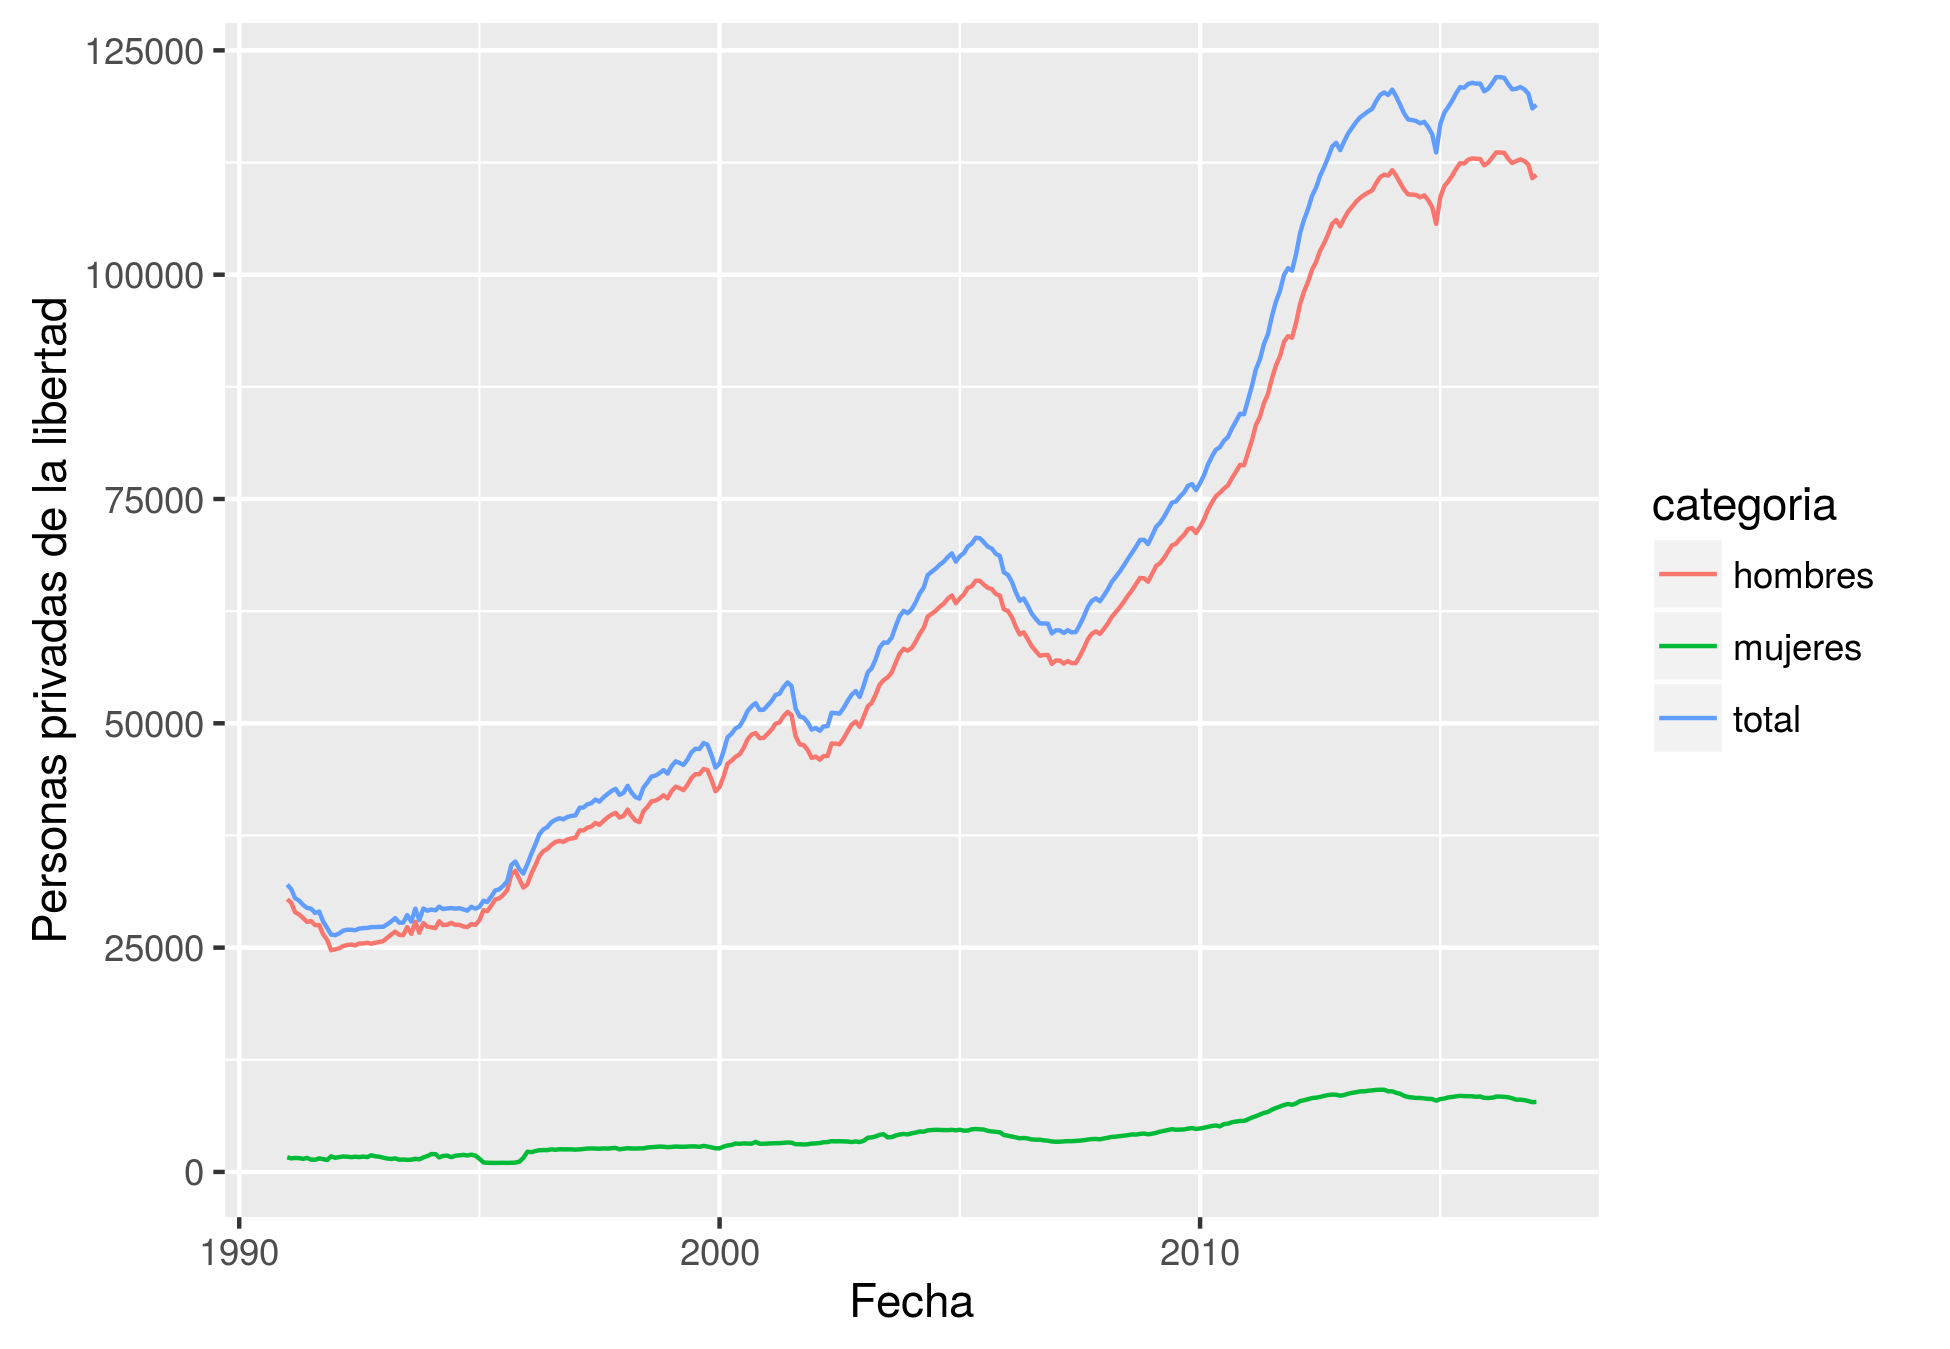
\includegraphics[width=10cm]{genero.png}
	\caption{Poblaci�n privada de la libertad 1991 - 2017} {Fuente: INPEC\\} {Elaboraci�n propia}
	\label{fig:genero}
\end{figure}

El incremento en la poblaci�n carcelaria podr�a tomarse como un efecto del crecimiento de la poblaci�n colombiana. Para validar este supuesto calculamos la tasa de encarcelamiento, que mide la cantidad de personas encarceladas por cada cien mil habitantes. Este indicador pas� de 92 personas por cada cien mil habitantes en enero de 1991 a 242 en enero de 2016. Tal incremento se puede ver tanto en hombres como en mujeres. Ver figura \ref{fig:tasas}. 


\begin{figure}[htb]
	\centering
	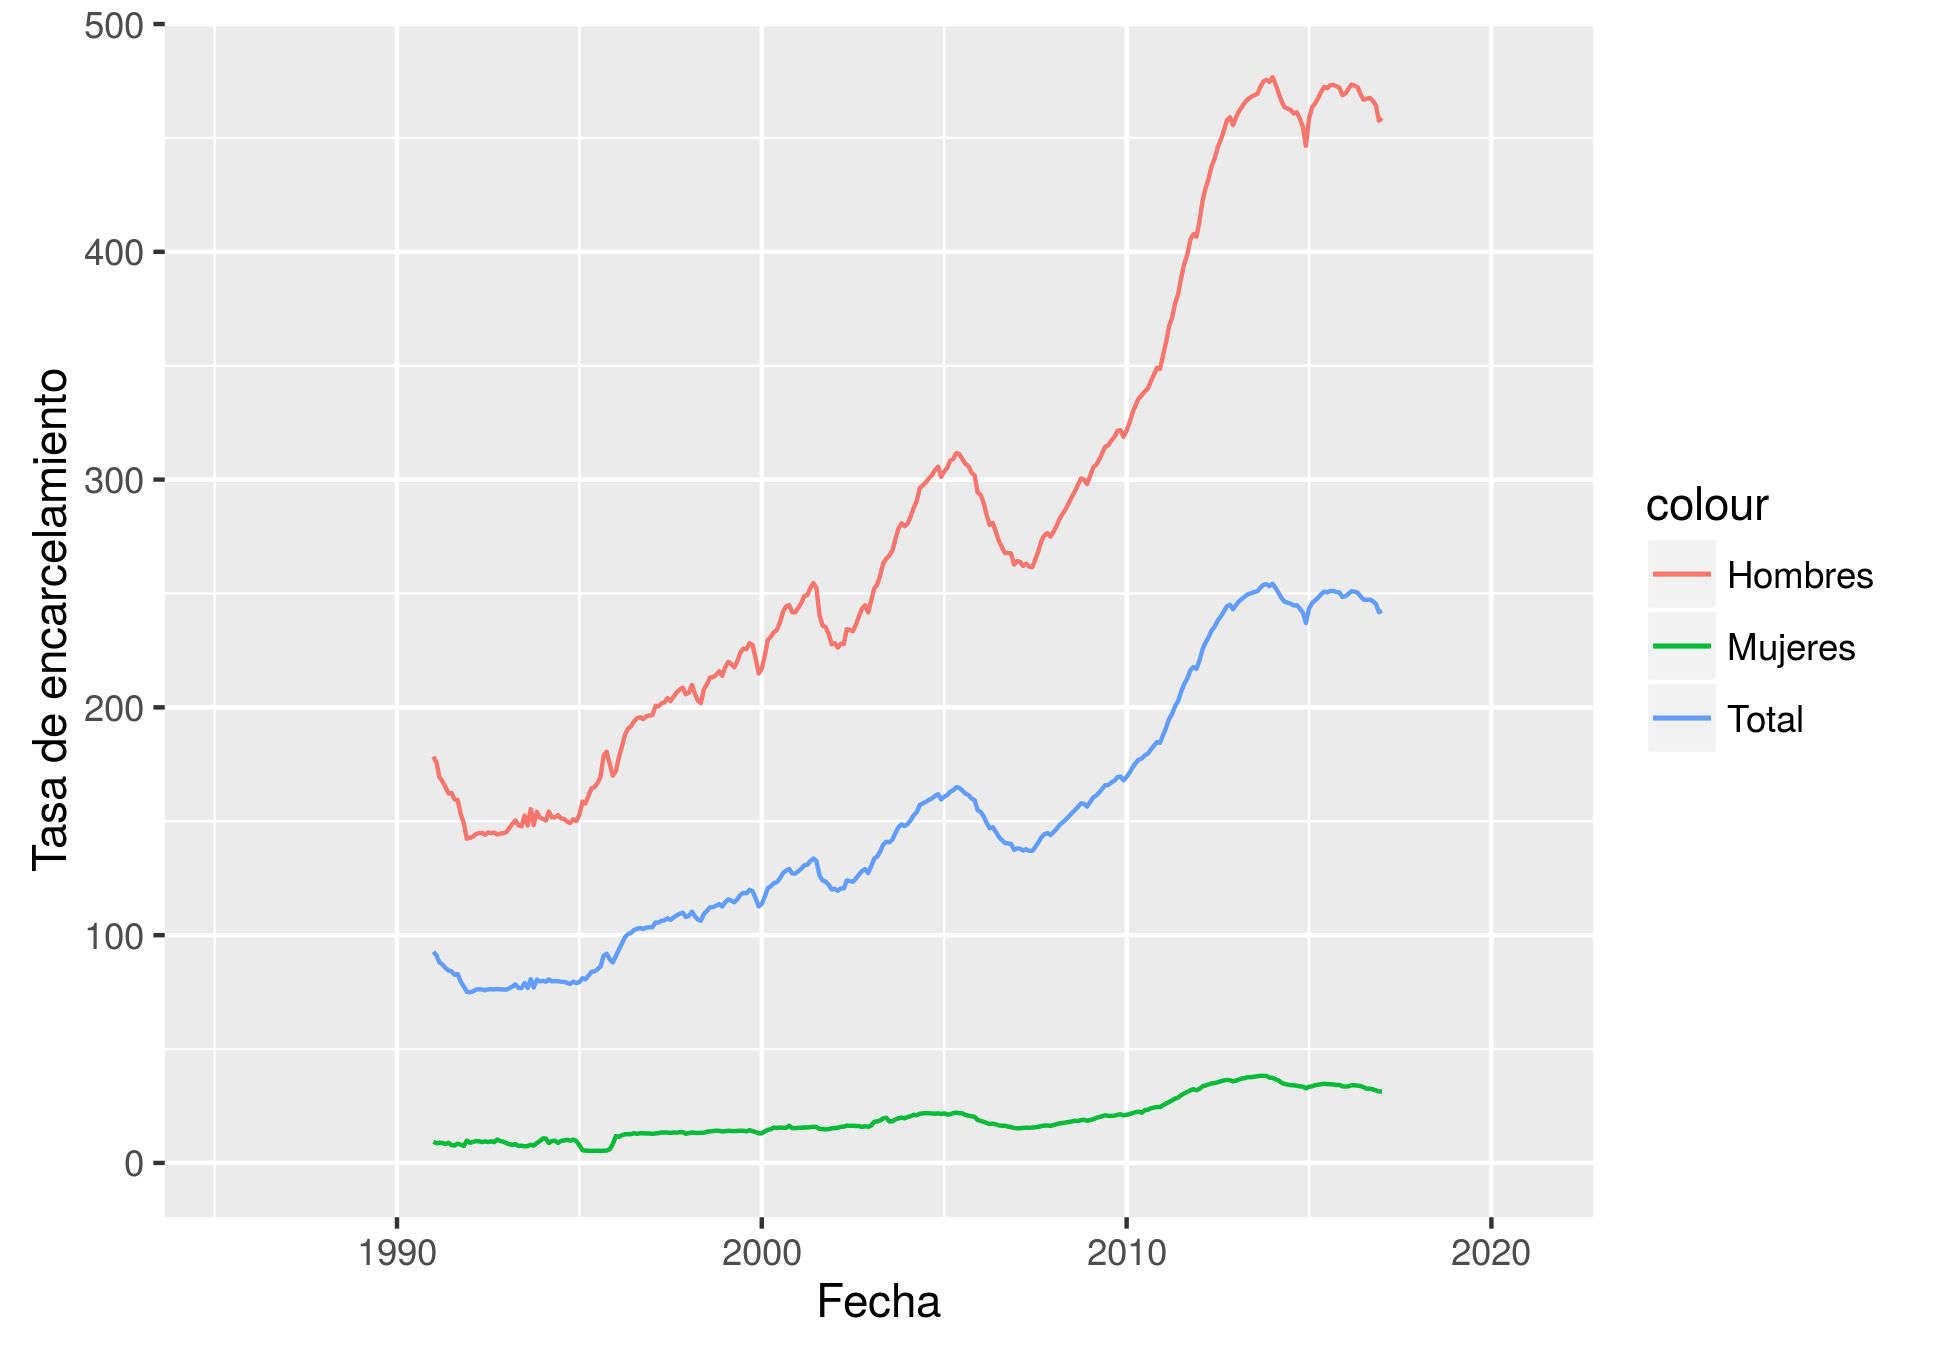
\includegraphics[width=10cm]{tasas}
	\caption{Tasa de encarcelamiento seg�n genero 1991 - 2017\\}{Fuente: INPEC\\} {Elaboraci�n propia}
	\label{fig:tasas}
\end{figure}

La tasa de encarcelamiento es un indicador que var�a seg�n la edad y genero, siendo m�s elevado en los hombres que en las mujeres y m�s algo en los hombres j�venes, que en los hombres mayores (cita pendiente).  Otra posible explicaci�n al cambio en la tasa de encarcelamiento es un cambio en la pir�mide poblacional en el periodo analizado. No obstante, no podemos confirmar o refutar esta hip�tesis pues la serie de tiempo, contenida en los datos de libre acceso no se encuentra desagregada por edad.

\section{El sistema penitenciario en Colombia}

La poblaci�n carcelaria se ve afectada por dos pol�ticas, la pol�tica penitenciaria, que determina las condiciones de privaci�n de la libertad y la pol�tica criminal que determina las causas de encarcelamiento y la duraci�n de las penas. \cite{DepartamentoNacionaldePlaneacion2015}

A la poblaci�n privada de la libertad antes del juicio se le denomina pobaci�n sindicada, y a aquellos que han sido juzgados y se encuentran cumpliendo la sentencia se les denomina poblaci�n condenada. La evoluci�n de la poblaci�n seg�n situaci�n jur�dica se puede observar en la figura \ref{fig:sit_jur}

\begin{figure}[htb]
	\centering
	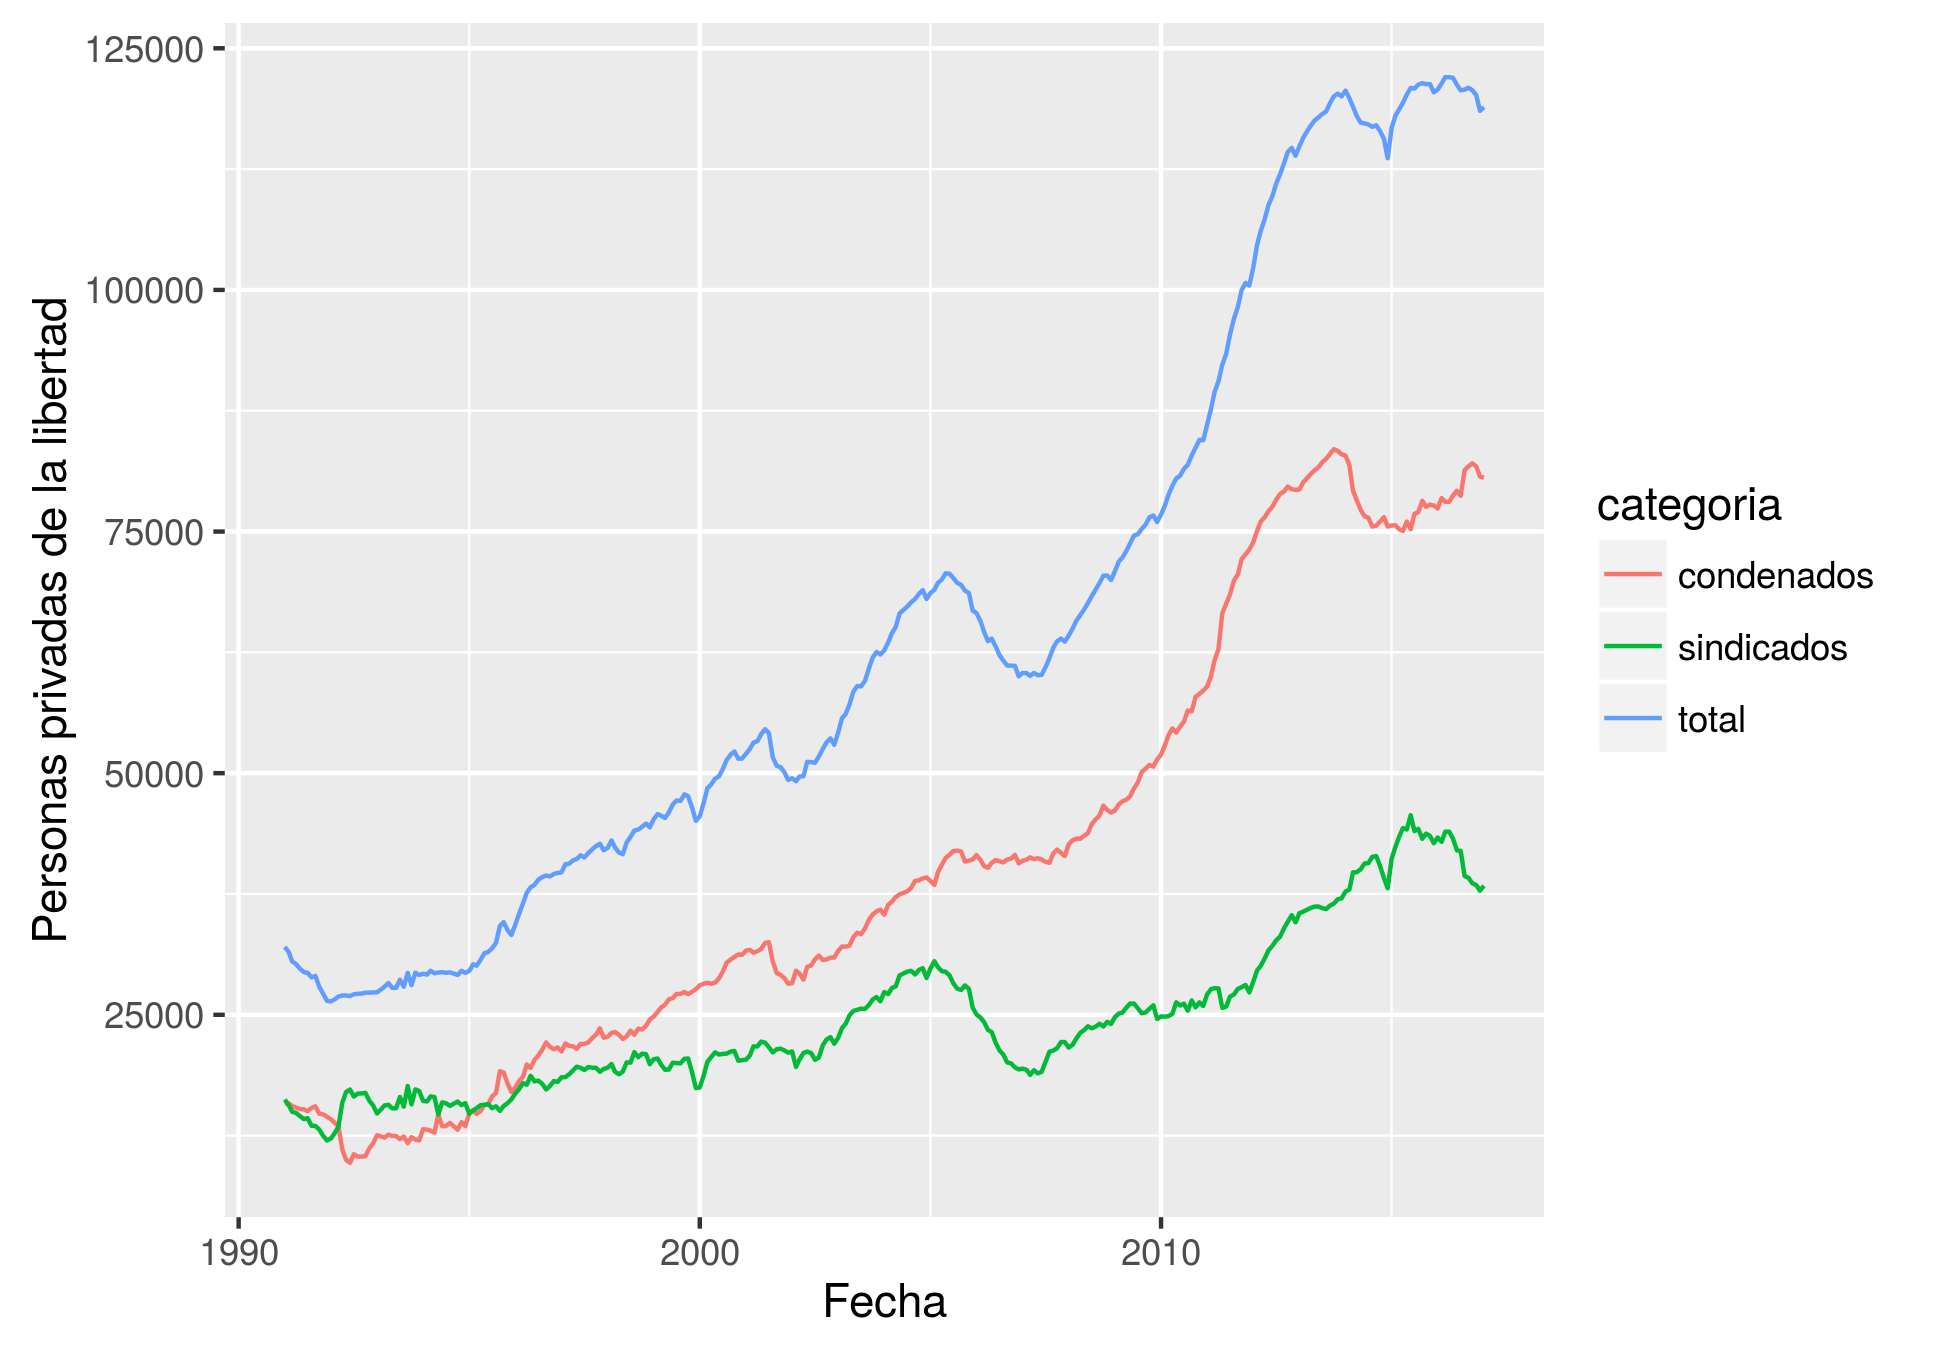
\includegraphics[width=10cm]{sit_jur.png}
	\caption{Poblaci�n carcelaria por situaci�n jur�dica\\} {Fuente: INPEC\\} {Elaboraci�n propia}
	\label{fig:sit_jur}
\end{figure}

\subsection{Identificaci�n del modelo}

Podemos modelar el sistema penitenciario de la siguiente manera:
%
\begin{equation}\label{Sindicados}
	S_t = S_{t-1} + \alpha {N_t} - \gamma S_{t-1}
\end{equation} 
%
\begin{equation}\label{Condenados}
	C_t = C_{t-1} - \omega C_{t-1} + \beta \gamma S_{t-1}
\end{equation} 
%
	$N_t$ = poblaci�n nacional en el periodo t \\
	$S_t$ = poblaci�n de sindicados en el periodo t\\
	$C_t$ = poblaci�n de condenados en el periodo t\\
	$\alpha$ = proporci�n de la poblaci�n libre que ingresa al sistema carcelario \\
	$\gamma$ = proporci�n de sindicados que es juzgada cada periodo \\
	$\beta$ = proporci�n de sindicados que han sido encontrados culpables durante el juicio	\\
	$\omega$ = proporci�n de condenados que cumplen su pena cada\\ periodo.
	
Y esto es un problema interesante porque no tengo las series de tiempo de la transici�n! 
	\chapter{Modelos SARIMA}

La estimaci�n de los modelos se realiza usando el paquete base del software R \cite{RCoreTeam2017}, y el paquete astsa \cite{Stoffer2014}, cuyo uso es discutido en detalle por Shumway \cite{Shumway}. 

En adelante nos referiremos a la funci�n de auctocorrelaci�n como ACF y a la funci�n de autocorrelaci�n parcial como PACF. 

\section{Identificaci�n del modelo}

% Variaci�n poblaci�n total, sindicada y condenada
\begin{figure}[H]
	\centering
	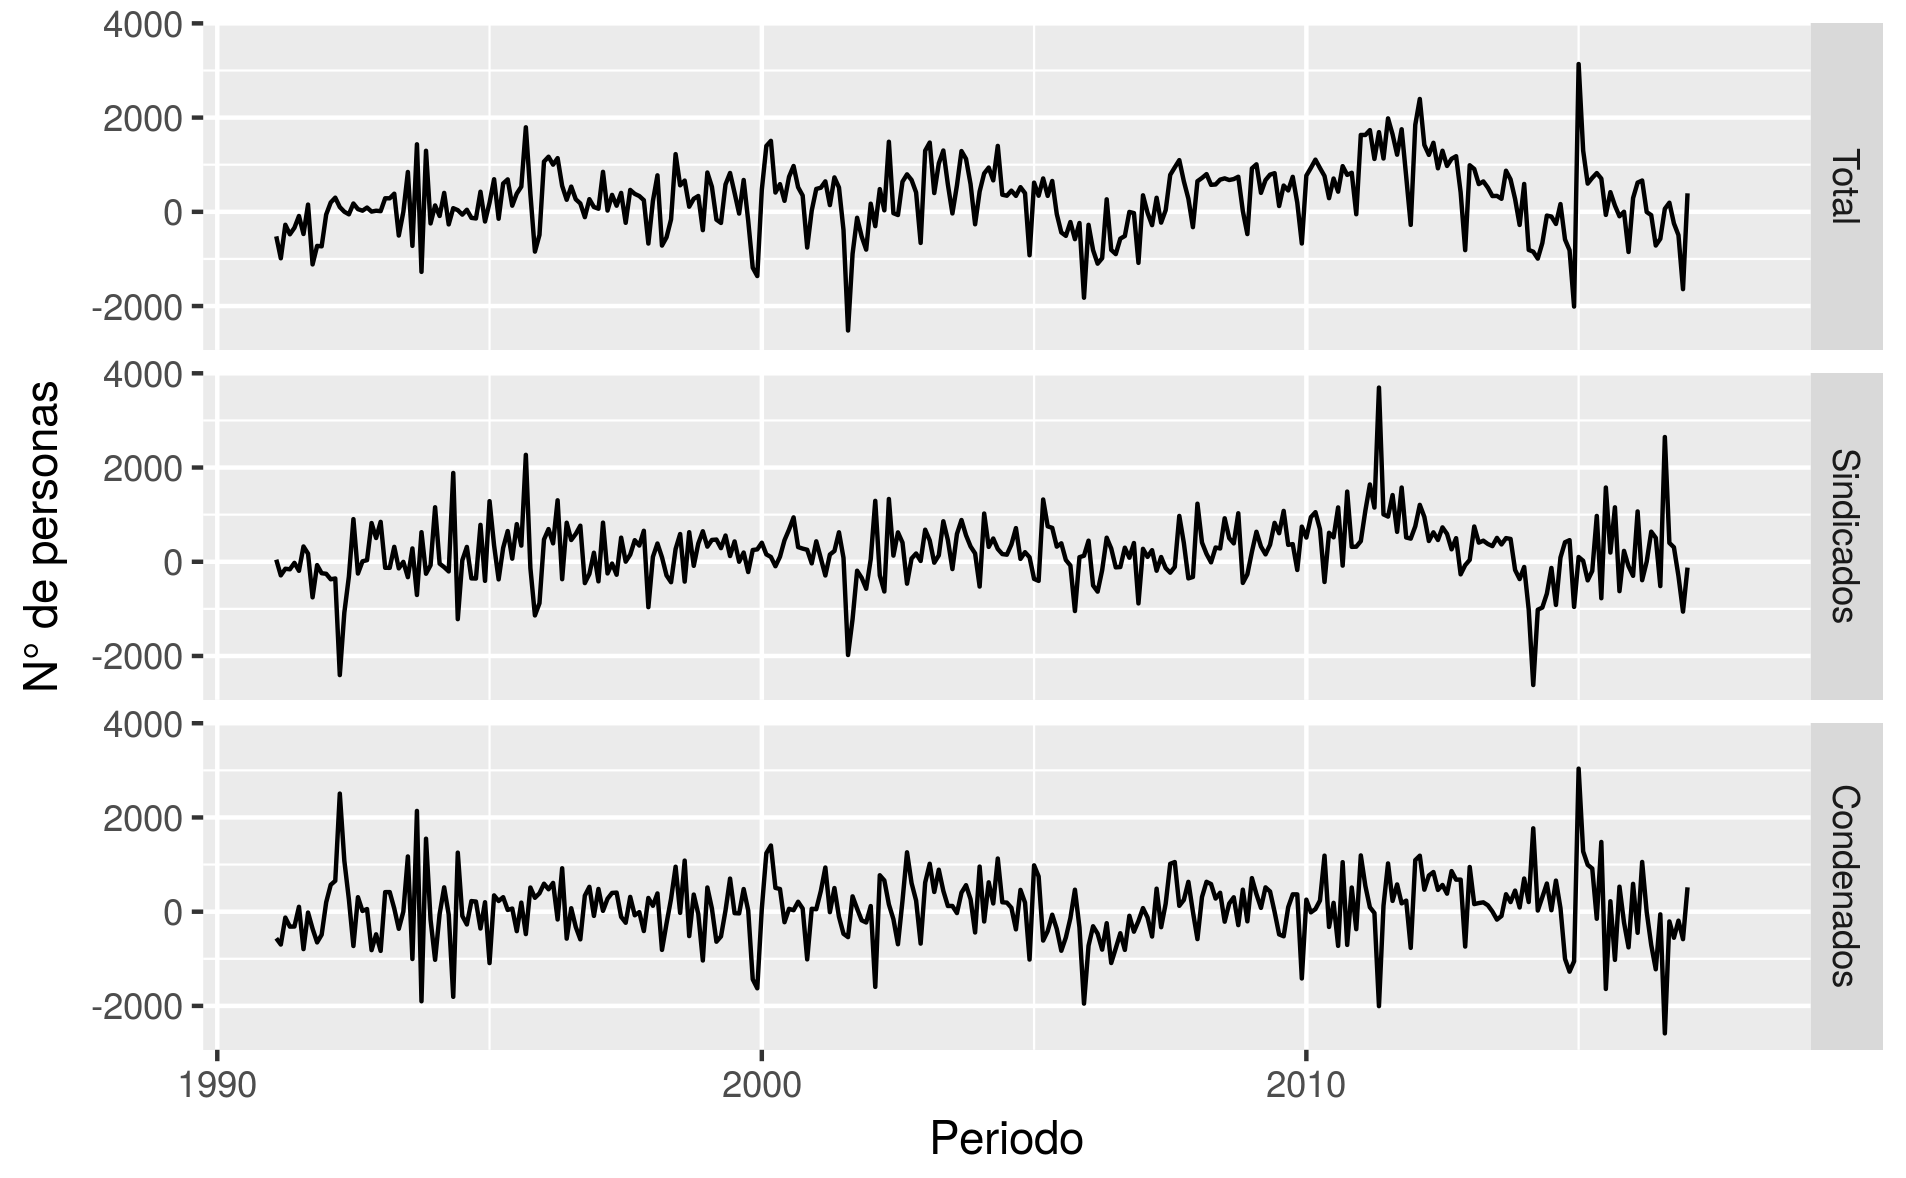
\includegraphics[width=0.7\linewidth]{variacion_intermensual}
	\caption[Variaci�n inter-mensual de poblaci�n carcelaria]{Variaci�n inter-mensual de poblaci�n carcelaria, sindicados y condenados}
	\label{fig:variacion_intermensual}
\end{figure}

Antes de realizar la proyecci�n de una serie de tiempo, es necesario identificar el modelo que explique adecuadamente su comportamiento. 

Aunque conocemos, por la estructura del proceso que genera los datos, que las series de tiempo de poblaci�n sindicada y condenada no son independientes, podemos simplificar la proyecci�n, trat�ndolas como independientes. En este caso, los modelos ARIMA y SARIMA resultan apropiados, pues permiten explicar separadamente cada observaci�n en funci�n del comportamiento hist�rico de la serie.

El cap�tulo anterior suger�a que la poblaci�n carcelaria, tanto sindicada como condenada, tiene una marcada tendencia al alza. En este caso una herramienta �til es mostrar gr�ficamente la variaci�n mes a mes de la poblaci�n. \ref{fig:variacion_intermensual}. Para tener una mejor estrucutura de an�lisis usamos la funci�n "decompose" de R base. 

La serie tiene un componente estacional marcado, con una reducci�n de la poblaci�n carcelaria en diciembre. La variabilidad del componente aleatorio es elevada. La tendencia parece tener cambios estructurales en algunos periodos, por ejemplo reducci�n de la poblaci�n carcelaria entre 2005-2007,  y 2012 - 2015, e incrementos de la poblaci�n de magnitud mayor al promedio entre 2008 y 2012.

La mayor parte de la variaci�n de la poblaci�n total se puede asociar con variaciones en a poblaci�n sindicada \ref{fig:variacion_mensual_sindicados_desc}. La poblaci�n condenada tiene una tendencia con una tendencia m�s estable.  \ref{fig:variacion_mensual_condenados_desc}

% Descomposici�n variaci�n poblaci�n total
\begin{figure}[H]
\centering
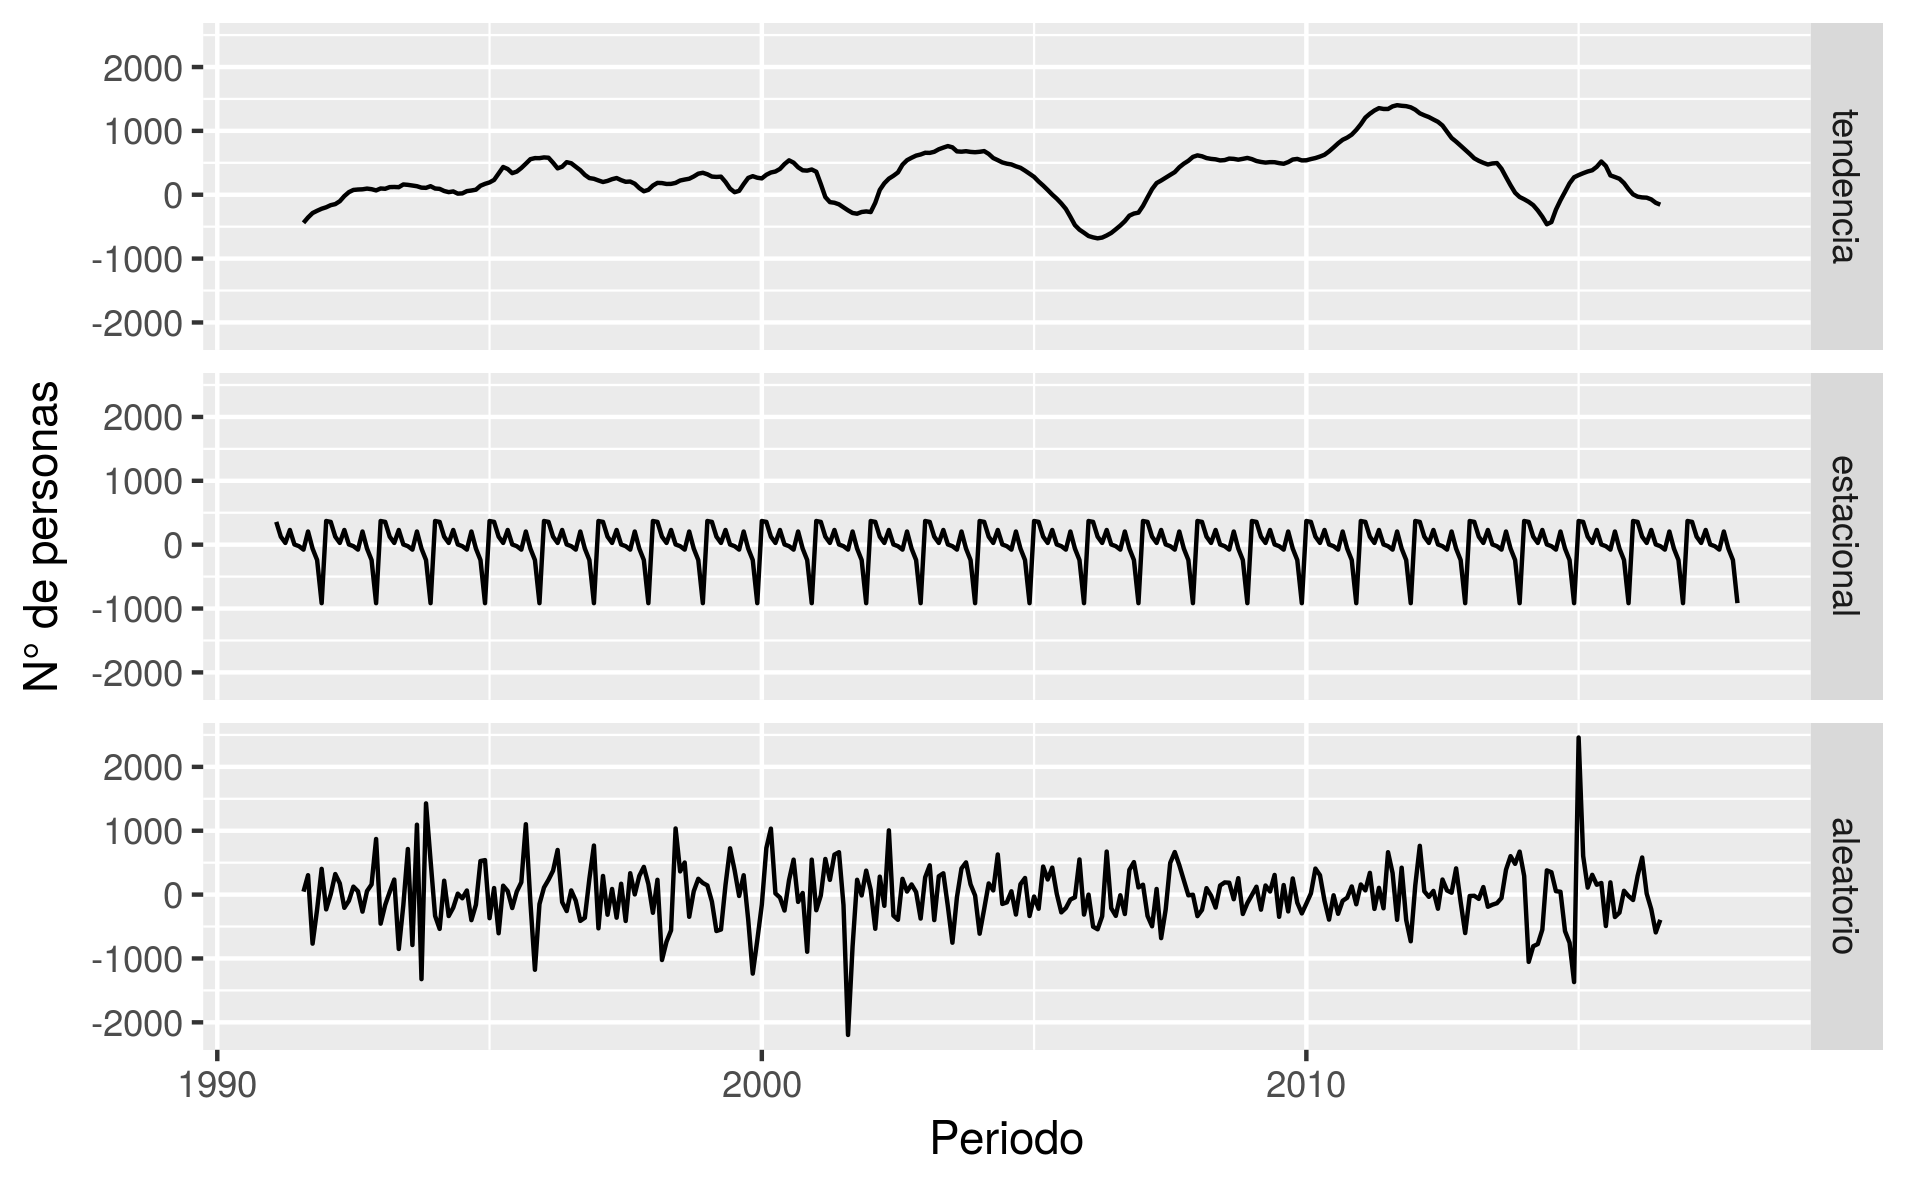
\includegraphics[width=0.7\linewidth]{variacion_mensual_total_desc}
\caption[Descomposici�n de la variaci�n inter-mensual de poblaci�n carcelaria total]{Variaci�n mensual de poblaci�n carcelaria descompuesta por tendencia, estacionalidad y componente aleatorio.}
\label{fig:variacion_mensual_total_desc}
\end{figure}

% Descomposici�n variaci�n poblaci�n sindicada
\begin{figure}[H]
	\centering
	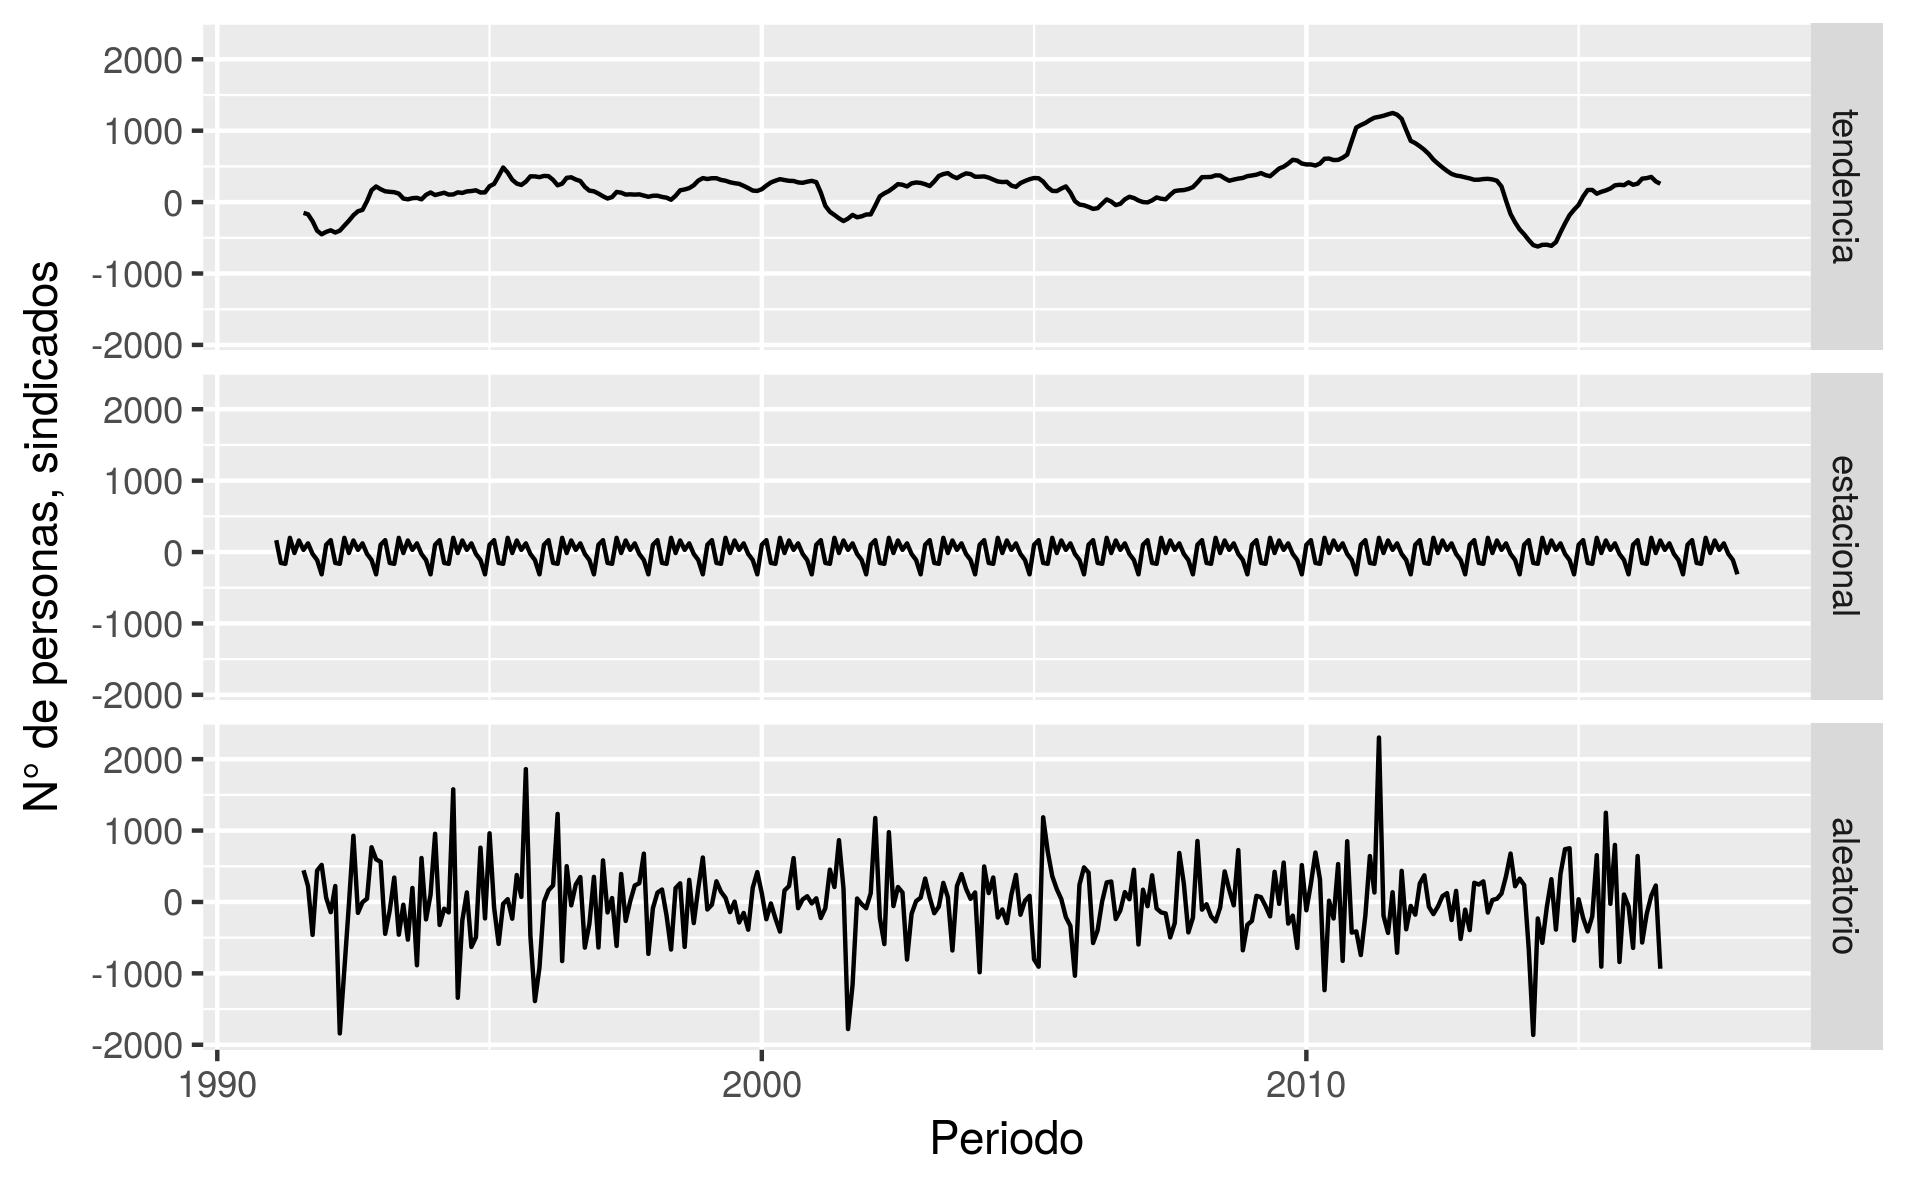
\includegraphics[width=0.7\linewidth]{variacion_mensual_sindicados_desc}
	\caption[Descomposici�n de la variaci�n inter-mensual de poblaci�n carcelaria total]{Variaci�n mensual de poblaci�n carcelaria sindicada,  descompuesta por tendencia, estacionalidad y componente aleatorio.}
	\label{fig:variacion_mensual_sindicados_desc}
\end{figure}

% Descomposici�n variaci�n poblaci�n condenada
\begin{figure}[H]
	\centering
	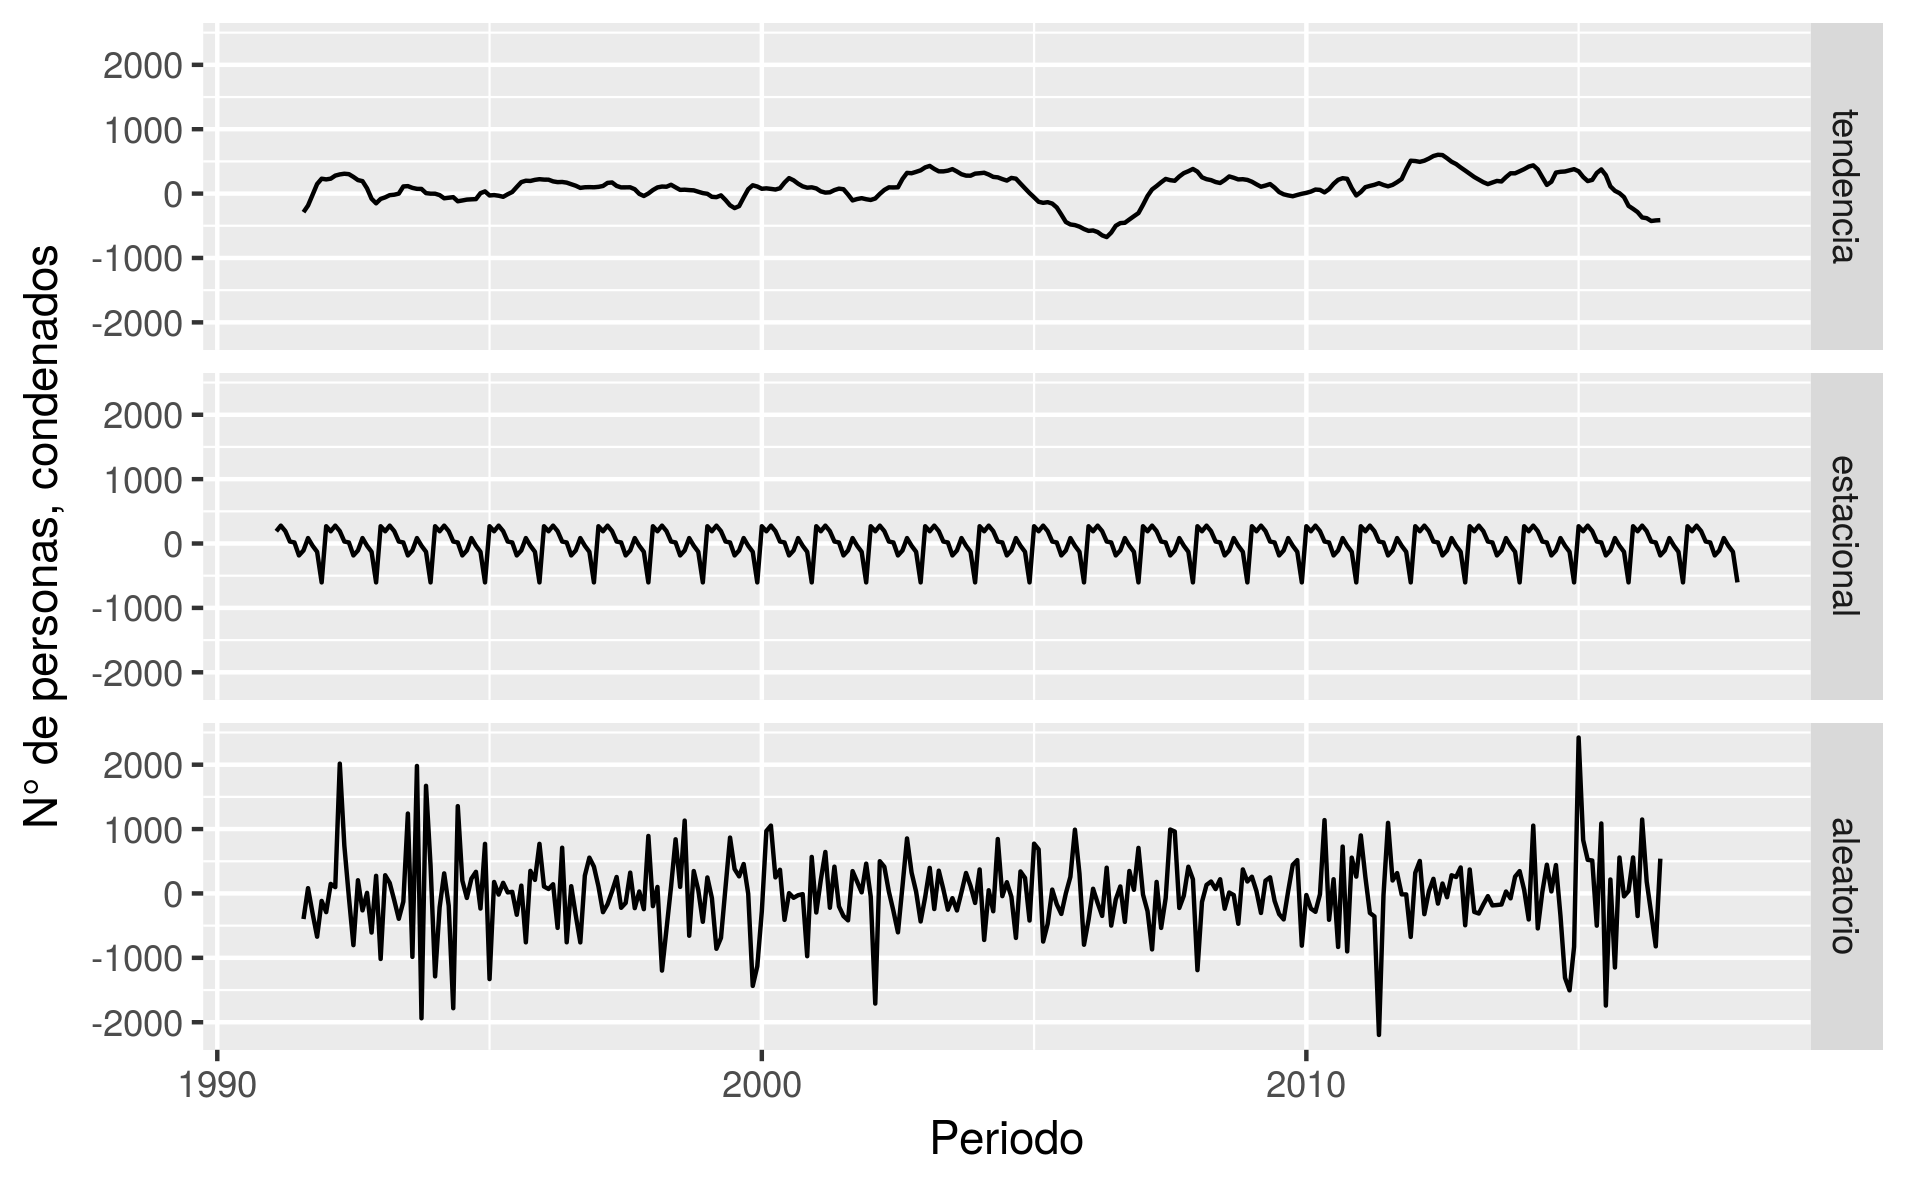
\includegraphics[width=0.7\linewidth]{variacion_mensual_condenados_desc}
	\caption[Descomposici�n de la variaci�n inter-mensual de poblaci�n carcelaria total]{Variaci�n mensual de poblaci�n carcelaria condenada,  descompuesta por tendencia, estacionalidad y componente aleatorio.}
	\label{fig:variacion_mensual_condenados_desc}
\end{figure}


Se trabaja sobre la diferencia de cada serie de tiempo con lag 1 y lag 12, al observar que la serie tiene un crecimiento sostenido entre 1991 y 2017, sugiriendo un proceso estocastico integrado. Sobre cada serie (poblaci�n total, poblaci�n sindicadda y poblaci�n condenada)  se realiza la funci�n de autocorrelaci�n y autocorrelaci�n parcial y se presenta en la figura \ref{fig:ACF_variacion_mensual}. Estas funciones son usadas como herramienta de diagn�stico, para intuir modelos adecuados en cada serie.

Con base en la tabla \ref{ARMA_ACF} se realiza una revisi�n del comportamiento de las series de poblaci�n carcelaria, poblaci�n sindicada y poblaci�n condenada.

% Pendiente traducir este fragmento
\begin{table}[H]
	\centering
	\caption{Comportamiento de la ACF y PACF en modelos ARMA(p,q) \cite{Shumway}}
	\label{ARMA_ACF}
	\begin{tabular}{lllll}
		\multicolumn{1}{|l|}{}              & \multicolumn{1}{c|}{\textbf{AR(p)}}       & \multicolumn{1}{c|}{\textbf{MA(q)}}       & \multicolumn{1}{c|}{\textbf{ARMA(p,q)}} &  \\ \cline{1-4}
		\multicolumn{1}{|l|}{\textbf{ACF}}  & \multicolumn{1}{l|}{Tails off}            & \multicolumn{1}{l|}{Cuts off after lag q} & \multicolumn{1}{l|}{Tails off}          &  \\ \cline{1-4}
		\multicolumn{1}{|l|}{\textbf{PACF}} & \multicolumn{1}{l|}{Cuts off after lag p} & \multicolumn{1}{l|}{Tails off}            & \multicolumn{1}{l|}{Tails off}          &  \\ \cline{1-4}
	\end{tabular}
\end{table}


\begin{figure}[H]
	\centering
	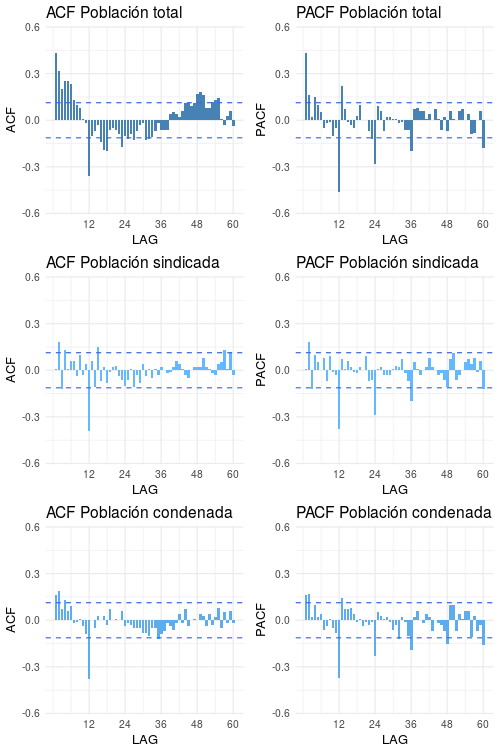
\includegraphics[width=0.7\linewidth]{ACF_var_pob}
	\caption[Autocorrelaci�n parcial de la variaci�n inter-mensual]{Autocorrelaci�n parcial de la variaci�n inter-mensual de la poblaci�n}
	\label{fig:ACF_variacion_mensual}
\end{figure}

\subsection{Poblaci�n total}

La tabla \ref{ARMA_ACF} presenta una gu�a para la interpretaci�n de la ACF y la PACF. En la \ref{fig:ACF_variacion_mensual} podemos observar que tanto la ACF como la PACF decaen lentamente. La APCF decae progresivamente en los meses 12, 24, 36, mientra que la ACF se corta en el lag 24, lo que sugiere que el proceso es un promedio m�vil de orden 1 en el componente estacional.

En este caso una primera estimaci�n se realiza para la proyecci�n de la poblaci�n total como SARIMA(1,1,1,0,0,1)


\subsection{Poblaci�n sindicada}

En la \ref{fig:ACF_variacion_mensual} podemos observar que la ACF decae lentamente, mientras la PACF cae por debajo del error luego del lag 1. La APCF decae progresivamente en los meses 12, 24, 36, mientra que la ACF se corta en el lag 12, lo que sugiere que el proceso es un promedio m�vil de orden 1 en el componente estacional.

En este caso una primera estimaci�n se realiza para la proyecci�n de la poblaci�n sindicada como SARIMA(1,1,1,0,0,1)

\subsection{Poblaci�n condenada}

El comportamiento de la ACF y la PACF es similar al de la poblaci�n sindicada, sugiriendo el mismo modelo: SARIMA(1,1,1,0,0,1).

\section{Estimaci�n de par�mtetros}
El proceso de estimaci�n se realizar� para cada serie por separado, luego se validar� la efectividad de incluir m�s par�metros, usando como criterio de comparaci�n el BIC. A modo informativo se usa la funci�n auto.arima del paquete forecast, para seleccionar el modelo con menor AIC. \cite{Hyndman2017}  
 \cite{Hyndman2008} 
 
\subsection{Poblaci�n total}

\subsection{Poblaci�n sindicada}

\subsection{Poblaci�n condenada}


\section{Proyecci�n}

\subsection{Poblaci�n total}

\subsection{Poblaci�n sindicada}

\subsection{Poblaci�n condenada}

\section{Conclusiones}

Al usar un ARIMA
	\chapter{M�todos demogr�ficos para poblaciones peque�as}

No todas las personas tenemos la misma probabilidad de ser encarceladas. Los hombres tienen tasas de encarcelamiento m�s altas que las mujeres, y las personas entre 18 y 40 a�os son m�s susceptibles que los mayores de 40 \cite{Blumstein1980a}. Las cifras  de encarcelamiento, presentadas en la figura \ref{fig:inpec_edad_genero1} sugieren que estas tasas son estables en periodos cortos de tiempo y proporcionales entre los diferentes rangos de edad (si el encarcelamiento en un rango de edad se eleva sucede un incremento proporcional en los otros).  

La poblaci�n colombiana ha cambiado significativamente desde 1991, tanto en su magnitud como en su composici�n por edad. Hemos pasado de 35 millones en 1991 a 45 millones en la segunda d�cada del siglo XXI. Tambi�n hemos presenciado una reducci�n en la proporci�n de menores de 18 a�os, que ha pasado de XXX en 1991 a XXX en 2016. Se proyecta que en 2020 tendremos tantas personas entre 15 y 29 a�os, como entre 0 y 14, cuando en 1991 la diferencia era del XXX \%. \cite{DANEPROY}

El grupo etario con mayor tasa de encarcelamiento est� entre los 18 y 29 a�os.  \cite{Blumstein1980a}. La poblaci�n total en este grupo crece sostenidamente en el periodo 1991-2020. Como porcentaje de la poblaci�n total, decrecen en dos puntos porcentuales en el mismo periodo, cediendo espacio a una poblaci�n de mayor edad. El crecimiento de este grupo etario, particularmente en hombres podr�a ser un buen predictor de la poblaci�n carcelaria.

Para incorporar la relaci�n entre la poblaci�n nacional y la poblaci�n carcelaria se recurre al m�todo censal-ratio,com�nmente usado en la proyecci�n de poblaciones peque�as. Este m�todo requiere la inclusi�n de variables sintom�ticas que agreguen informaci�n sobre la poblaci�n peque�a.

\begin{figure}[H]
	\centering
	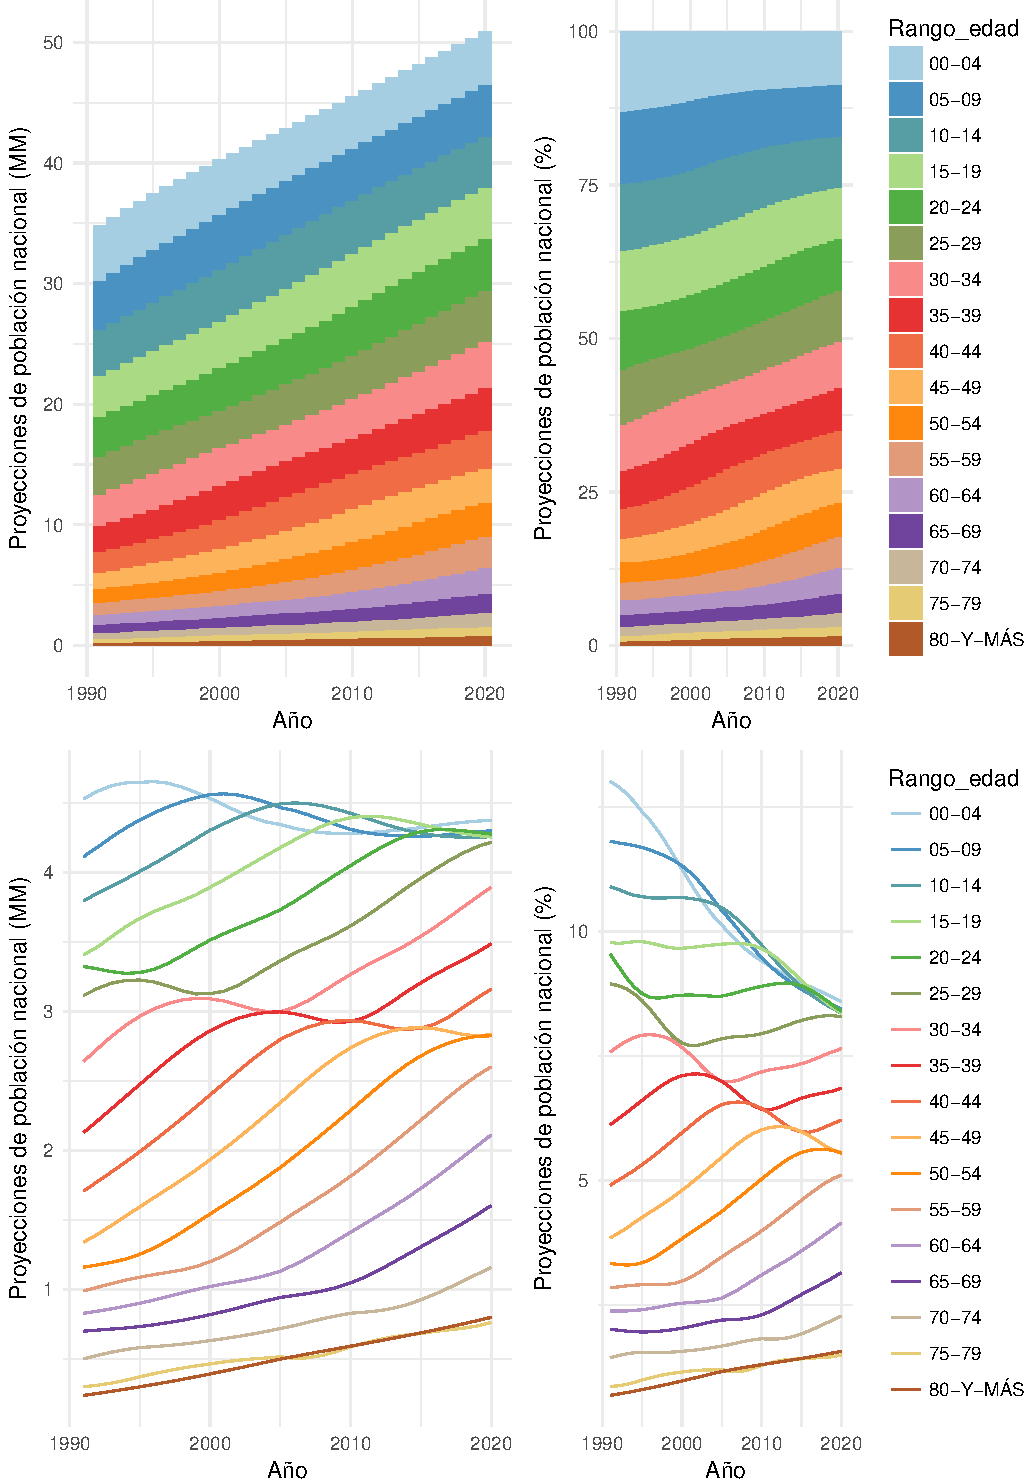
\includegraphics[width=0.9\linewidth]{POB_NAL_EDAD-1.pdf}
	\caption[Proyecci�n de la poblaci�n nacional por rango de edad]{Proyecci�n de la poblaci�n nacional por rango de edad}{Fuente: DANE} {Elaboraci�n propia}
	\label{fig:pob_nal_dane_edad}
\end{figure}


\section{Censal ratio}

Dentro de los m�todos para proyectar poblaciones peque�as se encuentra censal-ratio (raz�n-censal). �ste m�todo se vale una variable sintom�tica asociada a la poblaci�n peque�a, a la que se supone es directamente proporcional. Un ejemplo de variable sintom�tica es la cantidad de nacimientos en una ciudad, con respecto a su poblaci�n total; otro ejemplo es la cantidad de ni�os enrolados en un curso, con respecto a un rango etario en determinado espacio geogr�fico.

El censal-ratio supone que la relaci�n entre la variable sintom�tica y la poblaci�n a estimar es una variable aleatoria cuyo valor esperado no cambia a trav�s del tiempo. 

Cuando se cuenta con estimaciones independientes de la poblaci�n total en periodos inter-censales se realiza una correcci�n sobre las proyecciones de cada �rea, tal que la suma de las proyecciones de �reas peque�as sea igual a la estimada independientemente. La correcci�n mantiene la proporci�n entre proyecciones de �reas peque�as.

Un uso frecuente de los m�todos de proyecci�n para poblaciones peque�as es realizar interpolaci�n en periodos no censales. Uno de los inconvenientes mencionados es la dificultad de realizar extrapolaci�n, puesto que para los periodos post-censales, los indicadores no est�n necesariamente disponibles. Una posible soluci�n es realizar la estimaci�n usando periodos rezagados o utilizar la �ltima proyecci�n de la variable sintom�tica como proyecci�n. \cite{Swanson2012}. 

Siguiendo a Swanson \cite{Swanson2012} tenemos: 

$$ R_{A,t,j} = \frac{S_{A,t,j}}{P_{A,t}}$$

$ R $ = Raz�n entre variable sintom�tica y poblaci�n peque�a

$ A $ = A-�sima �rea peque�a

$ S $ = Valor de la variable sintom�tica

$ t $ = periodo

$ j $ = indicador

Si tenemos un R observado en el periodo T tendremos que la proyecci�n del periodo $t + k$ ser�:

$$ \hat{P}_{A,t+k} = \frac{S_{A,t + k ,j}}{R_{A,T,j}} $$

Cuando se tiene un estimado independiente para la poblaci�n padre se realiza un control, de manera que la suma de proyecci�n para las �reas peque�as sea igual a la proyecci�n del �rea padre: 

\begin{equation}
\hat{Q}_{A,t+k} = \frac{P_{A,t+k,j}}{\sum{P_{A,t+k,j}}} * P_{t+k}
\label{equ:inpec_edad_generotasa2}
\end{equation}

$\hat{Q}_{A,t+k}$ = Proyecci�n corregida para el �rea A 

$ P_{t+k}$ = Proyecci�n independiente total en el periodo $t + k$



La variable sintom�tica cumple la tarea de agregar informaci�n conocida al modelo para hacerlo m�s preciso. En un primer paso se considera la poblaci�n privada de la libertad una poblaci�n peque�a, dentro de la poblaci�n nacional. Dentro de las estad�sticas publicadas periodicamente por el INPEC no se han encontrado variables sintom�ticas que cubran m�s de dos a�os \cite{INPEC2018}, raz�n por la cual se realiza el siguiente proceso: se utiliza una constante en el lugar de la variable sintom�tica, lo que da lugar a una proyecci�n constante por edad genero; luego ajustamos la proyecci�n al total nacional por rango de edad proyectado por el DANE. Este modelo es equivalente a proyectar una tasa de encarcelamiento constante para cada rango de edad. Para el periodo 2017 - 2020 se utiliza la tasa de encarcelamiento.

Aunque no conocemos el comportamiento de la tasa de encarcelamiento espec�fica por edad, conocemos la poblaci�n carcelaria total y la tasa de encarcelamiento. Usamos el supuesto de proporci�n estable por rango etario, para ajustar la proyecci�n 2005 - 2016 a la poblaci�n carcelaria total.

$R_e = \frac{1} {P_{c,e, 2017}} $

$\hat{P}_{c, 2017 + k} = P{c, e, 2017}$

y 

$\hat{Q}_{c, e, 2017+k} = (\hat{P}_{c, e, 2017} * P_{e,2017}) * P_{e,2017 + k}$ 

donde: 

$\hat{Q}_{c, e, 2017+k}$ = Proyecci�n de poblaci�n carcelaria ajustada, para el rango etario, en el periodo $2017 + k$ 

$P_{c, 2017}$ = Poblaci�n carcelaria en 2017, a mitad de periodo, en el rango etario e.

$P_{e,2017}$ = Poblaci�n estimada 2017 DANE a mitad de periodo en el rango etario e. 

$P_{e,2017 + k}$ = Poblaci�n estimada en $2017 + k$, del DANE a mitad de periodo en el rango etario e.

Al aplicar esta proyecci�n a periodos anteriores a 2017 tenemos una estimaci�n de lo que habr�a sido la poblaci�n carcelaria, en un escenario de tasas de encarcelamiento espec�ficas constantes. Al comparar esta proyecci�n con la poblaci�n privada de la libertad observada, es posible evidenciar el impacto que ha tenido el proceso de cambio demogr�fico en la poblaci�n carcelaria, adem�s de poner en evidencia que no es el principal factor detr�s de este cambio. El incremento debe adem�s corresponder con un incremento de las tasas de encarcelamiento espec�ficas.

Para ajustar la proyecci�n de las tasas de encarcelamiento espec�ficas se trata la poblaci�n carcelaria como un �rea padre y a las poblaciones por rango etario como poblaciones peque�as. Usando la ecuaci�n \ref{equ:inpec_edad_generotasa2} tenemos: 

$$\hat{V}_{c, e, 2017+k} = (\hat{P}_{c, e, 2017} * \hat{P}_{c,2017+k}) * P_{c,2017 + k}$$

donde: 

$\hat{V}_{c, e, 2017+k}$ = Poblaci�n carcelaria ajustada por edad. 

$ \hat{P}_{c,2017+k}$ = Poblaci�n carcelaria estimada por genero.

$ P_{c,2017 + k} $ = Poblaci�n carcelaria observada. 

\section{Poblaci�n privada de la libertad por rango de edad Febrero 2016 a Febrero 2018}

El INPEC publica un reporte mensual con estad�sticas detalladas de la poblaci�n carcelaria al cierre de mes. Los reportes est�n disponibles en la p�gina del INPEC desde e incluyen la composici�n de la poblaci�n privada de la libertad desde Enero 2013. La estructura de los reportes no es uniforme para todos los periodos. La composici�n por rangos etarios antes de febrero 2016 consolidaba en las categor�as: 18 a 29 a�os, 29 a 54 a�os, 55 a 64 a�os, y mayor de 65 a�os. A partir de marzo de 2016 se agrupa 18 a 24 y grupos quinquenales hasta los 65 a�os. \cite{INPEC2018}

En la figura \ref{fig:inpec_edad_genero2} podemos observar la composici�n demogr�fica de la poblaci�n privada de la libertad en Junio 2017. Es una poblaci�n compuesta mayoritariamente por hombres. Tanto en hombres como mujeres se observa un patr�n similar en la estructura etaria, el punto m�s alto se encuentra entre 25 y 29 a�os, 18 a 25 y 29 a 35 tienen un orden de magnitud comparable. Despu�s de los 35 a�os la poblaci�n se reduce en cada grupo quinquenal. 

En la figura \ref{fig:inpec_edad_genero3} se presenta la poblaci�n privada de la libertad, separada por genero y edad desde marzo 2016 hasta marzo 2018. El periodo de an�lisis se escogi� a conveniencia, considerando la disponibilidad de datos del INPEC con grupos etarios uniformes. La figura \ref{fig:inpec_edad_genero3} muestra que la poblaci�n carcelaria mantiene la forma de campana, con pico en 25-29, en todos los meses analizados, tanto en hombres como mujeres. En hombres el rango de edad con mayor variabilidad es el rango 18-24. En mujeres la variabilidad se presetnta en los rangos 18-24, 25-29 y 30-34. \cite{Ram2018}


\begin{figure}[H]
	\centering
	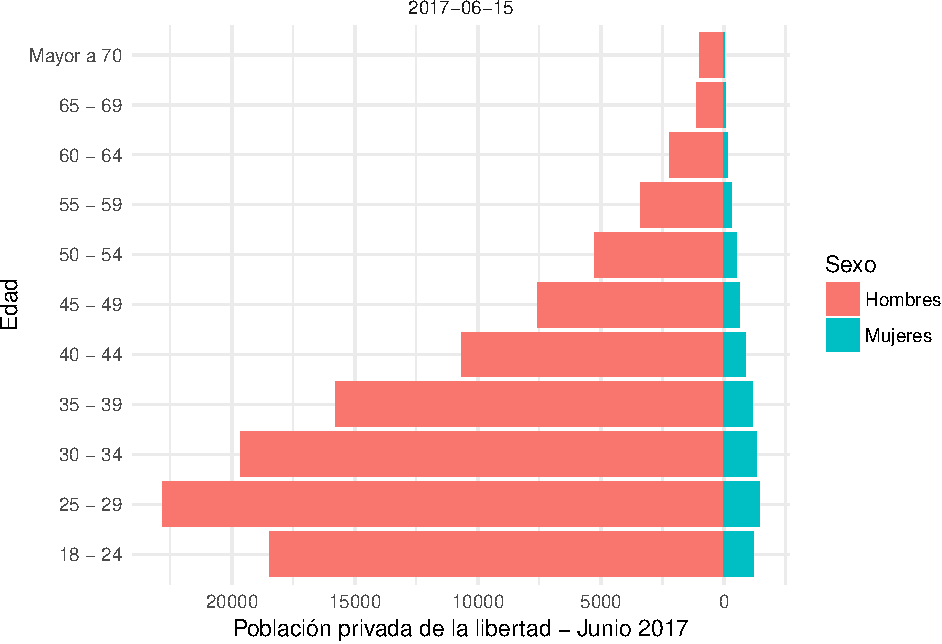
\includegraphics[width=0.7\linewidth]{gginpec_edad_genero2-1.pdf}
	\caption[Piramide poblacional, poblaci�n privada de la libertad, Junio - 2017]{Piramide poblacional, poblaci�n privada de la libertad, Junio - 2017}{Fuente: INPEC} {Elaboraci�n propia}
	\label{fig:inpec_edad_genero2}
\end{figure}


\begin{figure}	
	\centering
	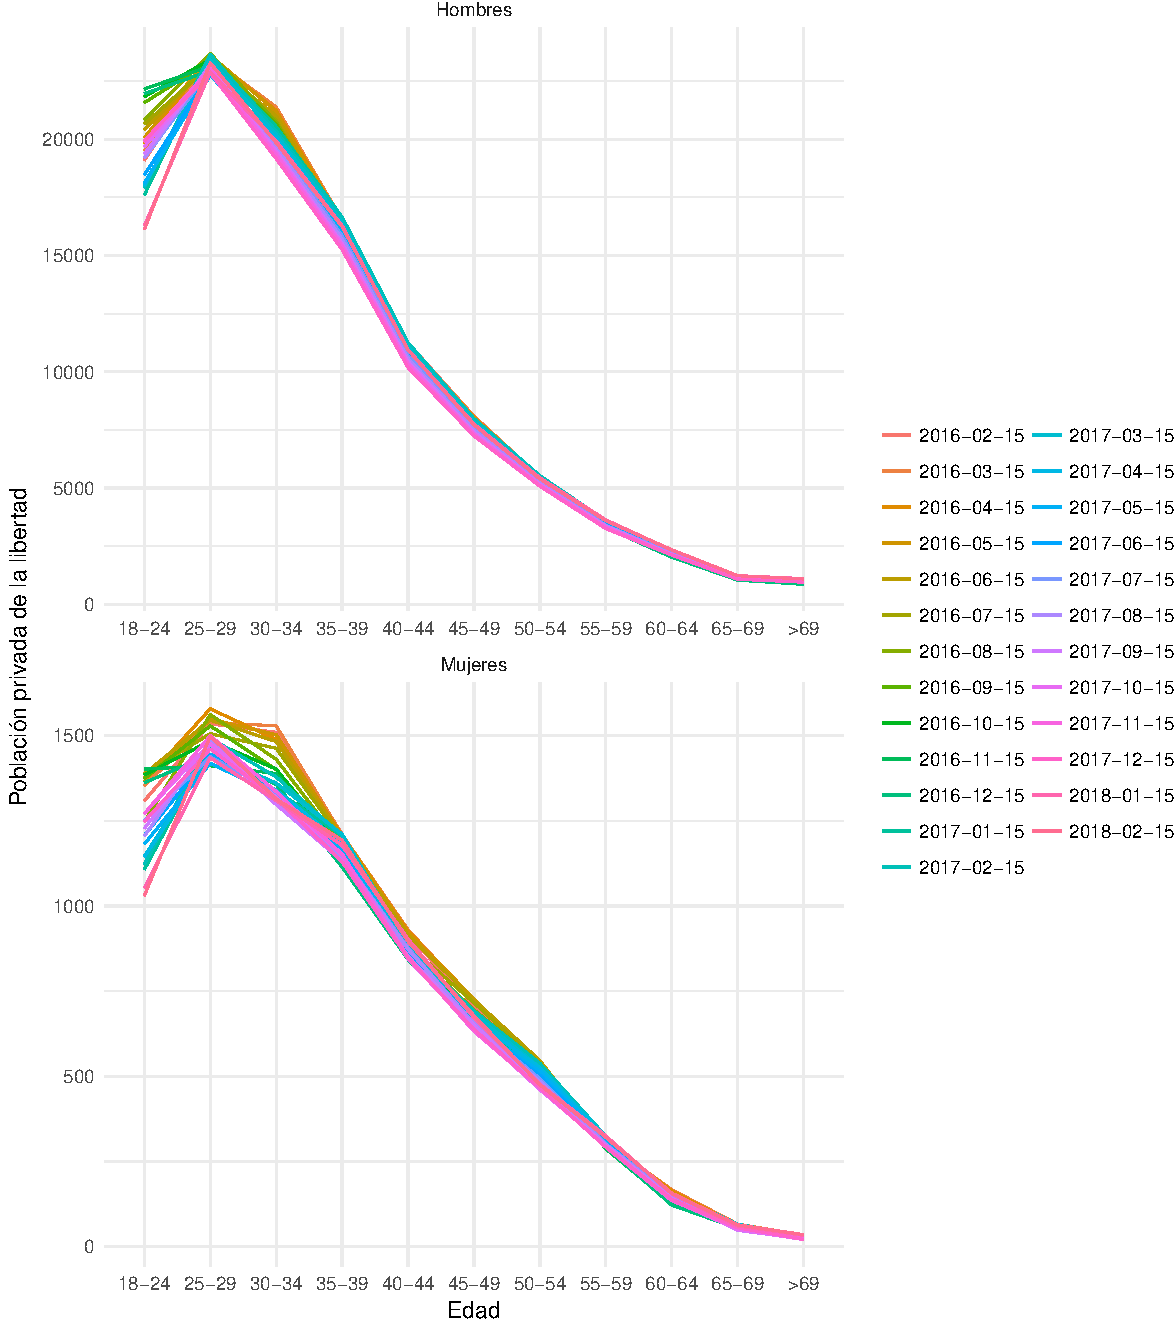
\includegraphics[width=0.7\linewidth]{inpec_edad_genero3-1.pdf}
	\caption[Poblaci�n privada de la libertad. Febrero-2016 a Febrero-2018]{Poblaci�n privada de la libertad. Febrero-2016 a Febrero-2018}{Fuente: INPEC} {Elaboraci�n propia}
	\label{fig:inpec_edad_genero3}
\end{figure}

Esta variabilidad podr�a estar asociada a un componente estacional o a un componente aleatorio. Aunque la longitud de la serie disponible no permite realizar inferencia sobre componentes de estacionalidad y tendencia, la figura muestra que: A trav�s del a�o el grupo 18-24 crece, para caer abruptamente en enero del a�o siguiente; comportamiento repetido en enero 2016 y enero 2017. El comportamiento es similar en mujeres una vez se controla por el orden de magnitud. El comportamiento en las dem�s series es similar, se reduce durante todo el a�o, para subir nuevamente en enero. Este comportamiento es coherente en hombres y mujeres, una vez se controla la magnitud. \ref{fig:inpec_edad_genero3} Este comportamiento implica que no es conveniente trabajar la proyecci�n de la tasa de encarcelamiento a nivel mensual pues no se puede estimar el aparente componente de estacionalidad de la serie. Por conveniencia se trabaja con la proyecci�n de poblaci�n a mitad de periodo, y se trata la tasa de encarcelamiento como una variable aleatoria cuyo valor esperado se mantiene a trav�s del tiempo.

\begin{figure}[H]
	\centering
	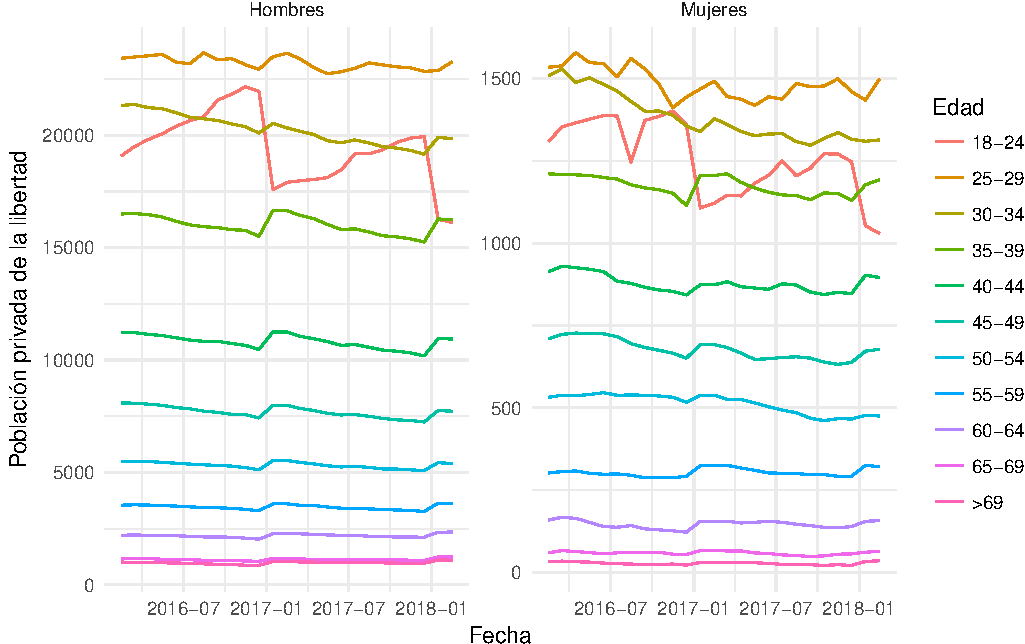
\includegraphics[width=0.7\linewidth]{inpec_edad_genero1-1.pdf}
	\caption[Poblaci�n privada de la libertad. Febrero-2016 a Febrero-2018]{Poblaci�n privada de la libertad por rango etario. Febrero-2016 a Febrero-2018}{Fuente: INPEC} {Elaboraci�n propia}
	\label{fig:inpec_edad_genero1}
\end{figure}

Puesto que no se cuenta con informaci�n de periodos m�s extensos se valida an�lisis a un menor nivel de granularidad. Dentro de la informaci�n disponible se encuentra separada la poblaci�n carcelaria por regional. En la figura \ref{fig:inpec_edad_generoregion2} se observa nuevamente, en todas las regionales, la poblaci�n carcelaria con forma de campana. Consistentemente las mujeres tienen mayor variabilidad que los hombres en cada rango de edad y poblaciones carcelarias m�s peque�as se encuentran asociadas a una mayor variabilidad.

La forma del aparente componente estacional tambi�n se replica a nivel regional. Ver figura \ref{fig:inpec_edad_generoregion3}. 

\begin{figure}[H]
	\centering
	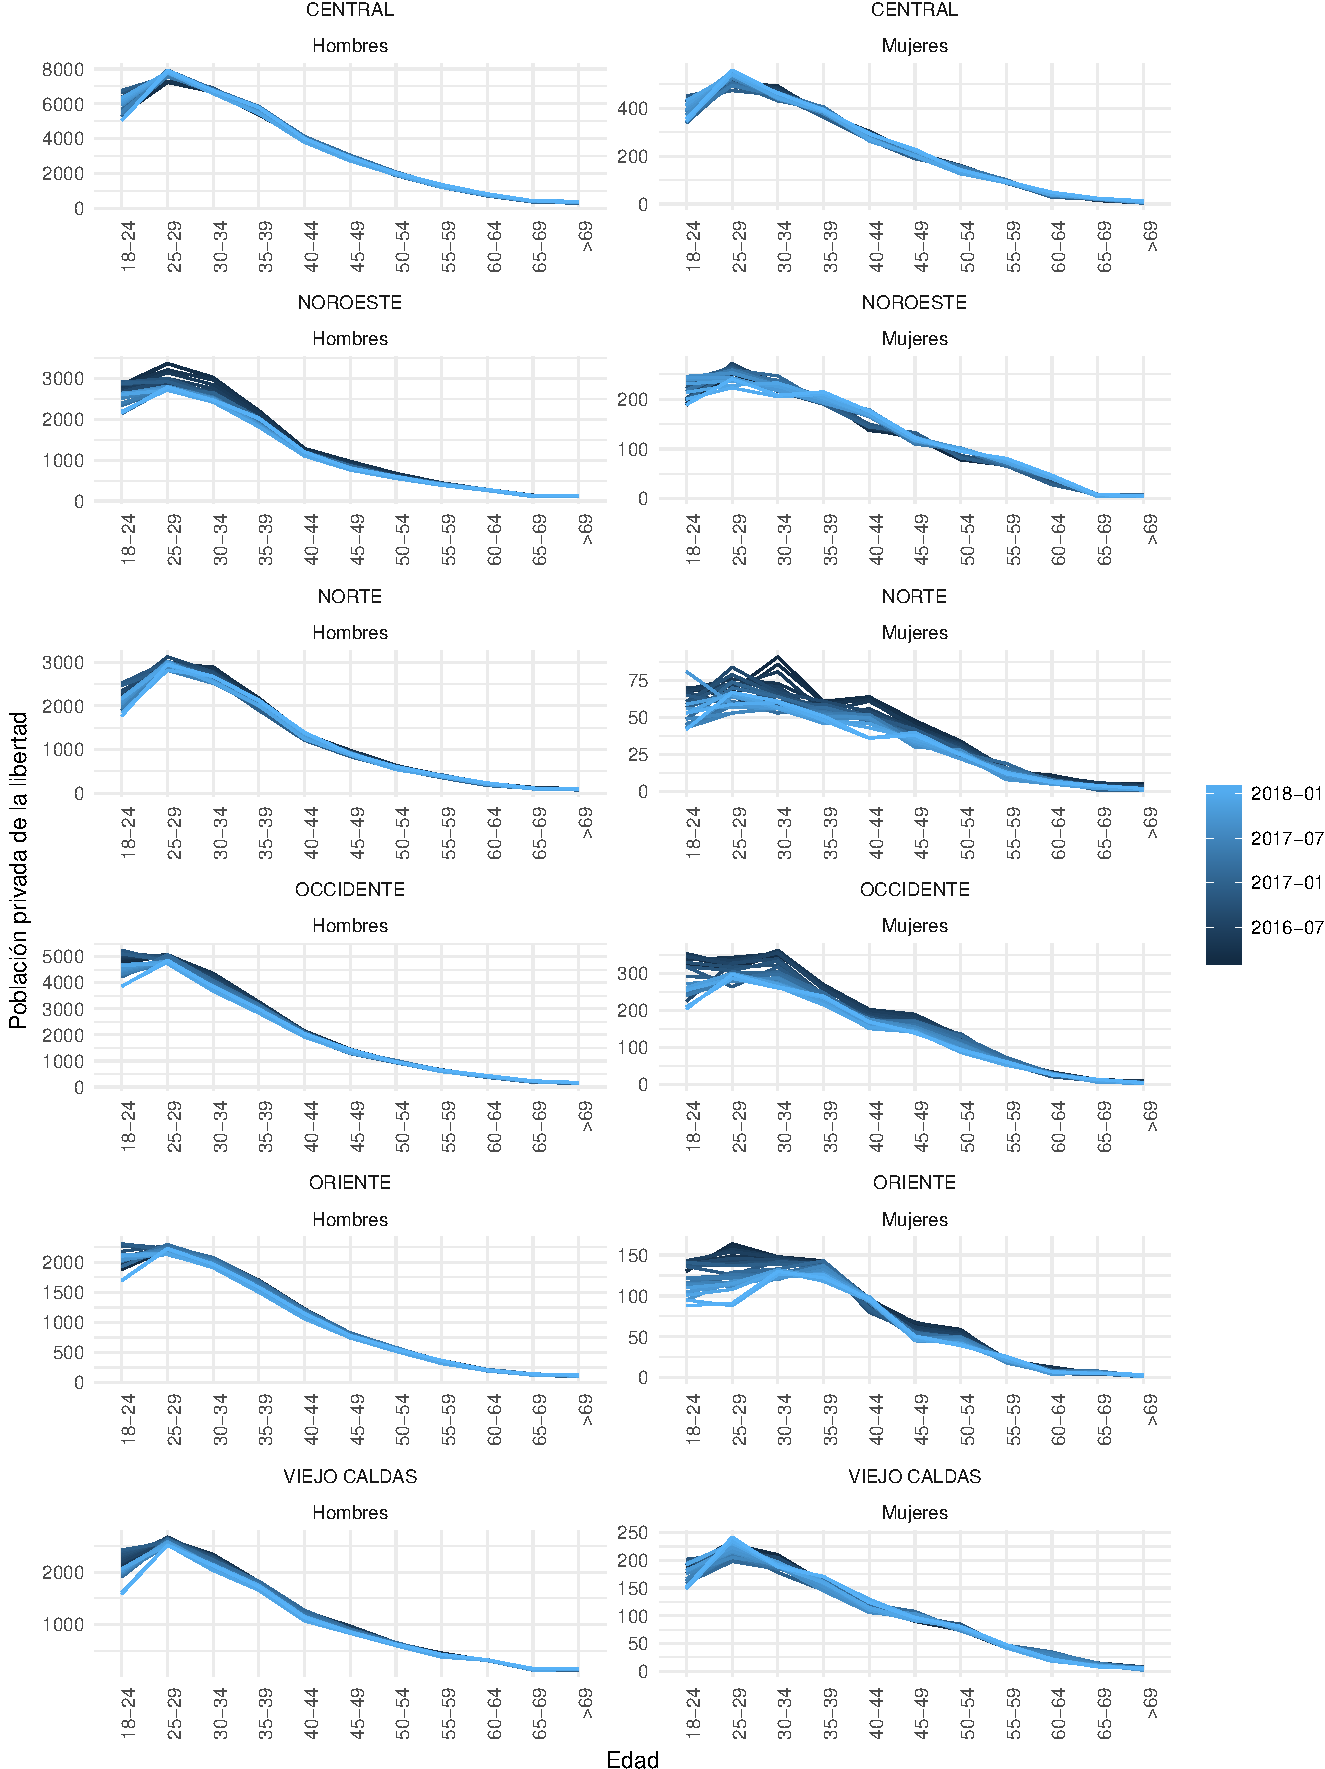
\includegraphics[width=1.1\linewidth]{inpec_edad_generoregion2-1.pdf}
	\caption[Poblaci�n privada de la libertad. Febrero-2016 a Febrero-2018]{Poblaci�n privada de la libertad por rango etario, regi�n. Febrero-2016 a Febrero-2018}{Fuente: INPEC} {Elaboraci�n propia}
	\label{fig:inpec_edad_generoregion2}
\end{figure}

\begin{figure}[H]
	\centering
	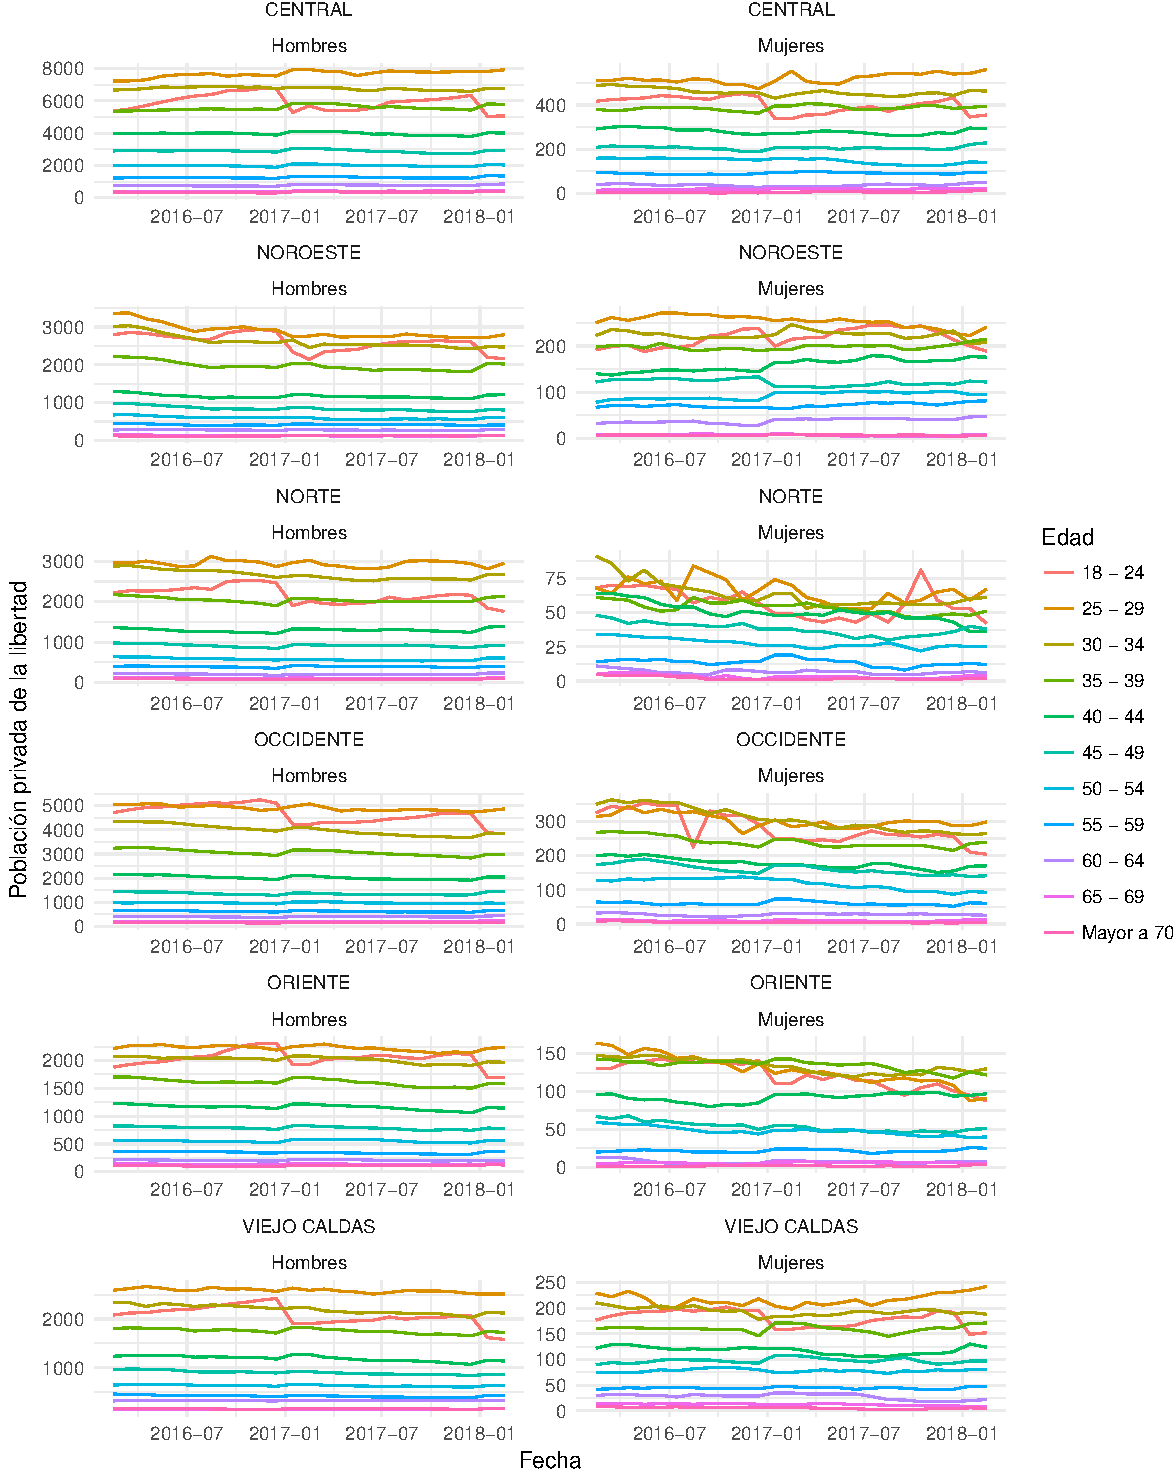
\includegraphics[width=1.1\linewidth]{gginpec_edad_genero_region-1.pdf}
	\caption[Poblaci�n privada de la libertad. Febrero-2016 a Febrero-2018]{Poblaci�n privada de la libertad por rango etario, regi�n. Febrero-2016 a Febrero-2018}{Fuente: INPEC} {Elaboraci�n propia}
	\label{fig:inpec_edad_generoregion3}
\end{figure}

Las personas no aparecen de la nada en la carcel. 


\begin{figure}[H]
	\centering
	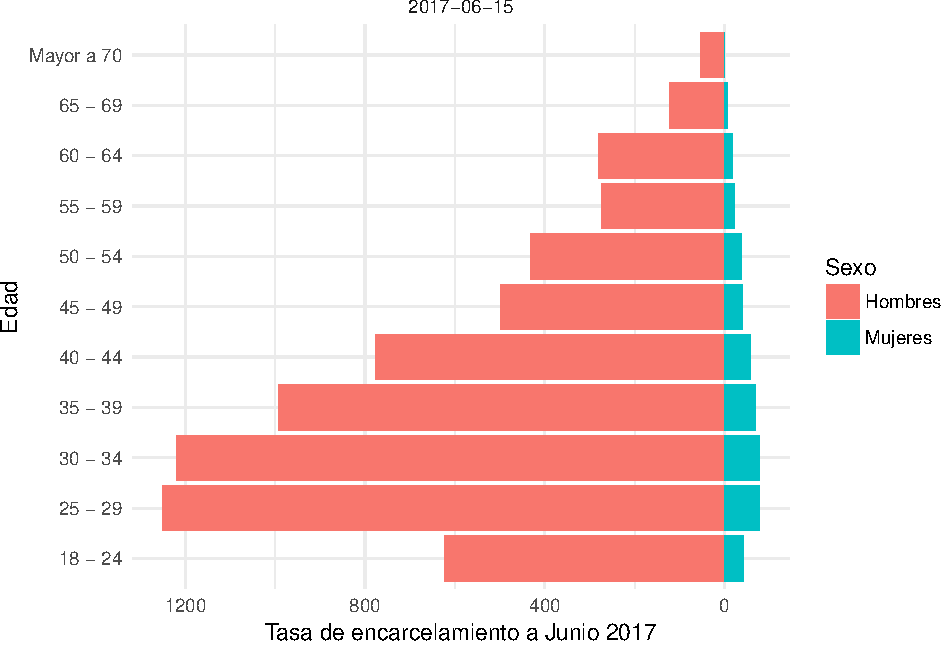
\includegraphics[width=0.7\linewidth]{gginpec_edad_generotasa1-1.pdf}
	\caption[Tasa de espec�fica de encarcelamiento. Junio-2017]{Tasa de espec�fica de encarcelamiento. Junio-2017}{Fuente: INPEC, DANE} {Elaboraci�n propia}
	\label{fig:inpec_edad_generotasa1}
\end{figure}

\begin{figure}[H]
	\centering
	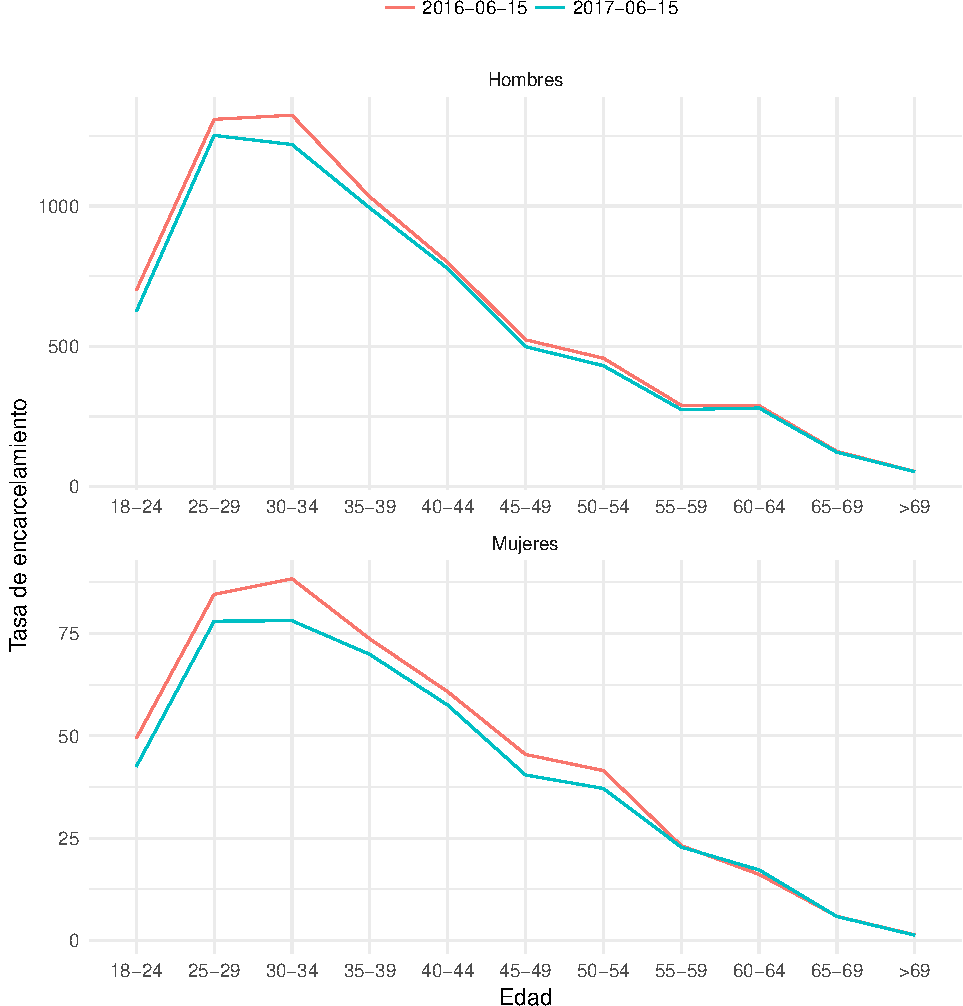
\includegraphics[width=0.7\linewidth]{inpec_edad_generotasa2-1.pdf}
	\caption[Tasa espec�fica de encarcelamiento. Junio-2016, Junio -2017]{Tasa espec�fica de encarcelamiento. Junio-2016, Junio -2017}{Fuente: INPEC, DANE} {Elaboraci�n propia}
	\label{fig:inpec_edad_generotasa2}
\end{figure}

\section{Proyecciones Censal Ratio}

\begin{figure}[H]
	\centering
	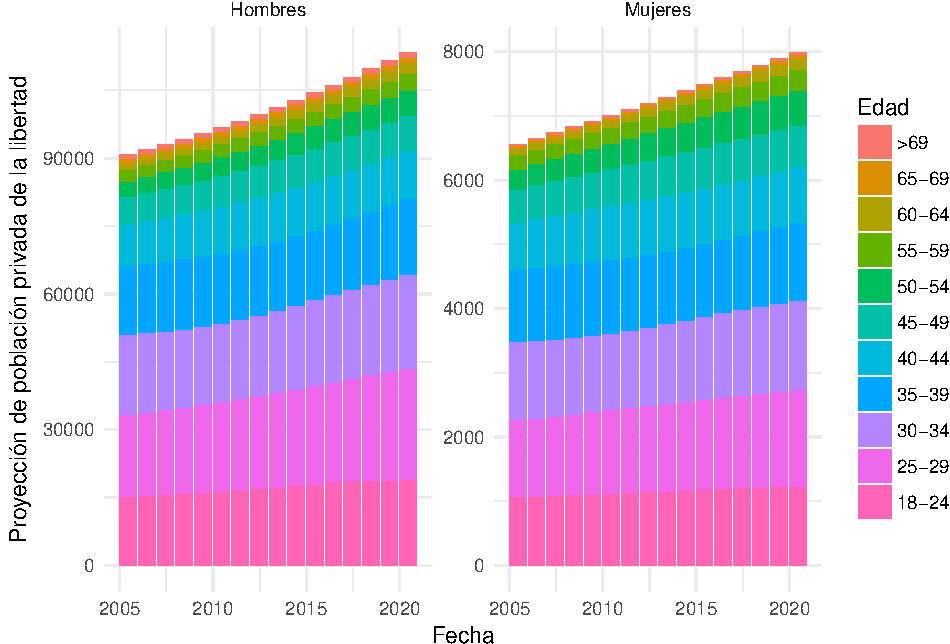
\includegraphics[width=0.9\linewidth]{Proyecciones_DANE-1.pdf}
	\caption[Poblaci�n privada de la libertad. 2005-2020]{Proyecci�n de la poblaci�n privada de la libertad,  2005 - 2020, ajustado por rango etario DANE}{Fuente: INPEC, DANE} {Elaboraci�n propia}
	\label{fig:inpec_edad_pry}
\end{figure}



	\chapter{Modelos Estado-Espacio}

El comportamiento de la poblaci�n carcelaria es diferente seg�n el delito y tiene relaci�n con un componente demogr�fico y un componente normativo. El componente demogr�fico se ha tratado en el cap�tulo anterior, en este cap�tulo se aborda el comportamiento de delitos. La interacci�n entre ambos no ha sido analizada pues no se cuenta con la informaci�n necesaria.

Las personas que se encuentran a la espera de juicio se llaman sindicados, y condenados quienes ya han recibido una sentencia. Cada mes una proporci�n de las personas sindicadas es sentenciada, puede entonces salir en libertad o cambiar a condenado, y una proporci�n de los condenados sale en libertad. Tambi�n se pueden presentar salidas por mortalidad. Un modelo auto-regresivo bivariado para la poblaci�n total puede modelar estas interacciones; particularmente la poblaci�n privada de la libertad est� compuesta por series separadas de diferentes delitos, cada una con un comportamiento diferente, como lo sugieren la figuras \ref{fig:delitoshombres} y \ref{fig:delitosmujeres}. 

Se presentan el comportamiento de la poblaci�n carcelaria por delito y g�nero. Con esta informaci�n se estima un modelo estado-espacio en cada una de las series bivariadas. Los modelos estado-espacio se formulan de forma tal que permitan modelar la interacci�n entre la poblaci�n sindicada y condenada.

\section{Poblaci�n privada de la libertad 2013-2016 por delito}

El INPEC incluye en sus estad�sticas mensuales la poblaci�n privada de la libertad separada por delito, estado (sindicado, condenado) y g�nero. Se ha consolidado la informaci�n disponible en reportes individuales entre Julio 2013 y Diciembre 2016, en una sola base de datos. Octubre 2015 se considera un dato faltante, pues a la fecha de descarga el reporte no se encuentra disponible en la p�gina del INPEC, \cite{INPEC2018}

En diciembre de 2016 la base de poblaci�n privada de la libertad por delito contaba con 184.116, frente a  una poblaci�n carcelaria de 118.532 individuos, en el mismo periodo. Esta diferencia se presenta pues un mismo individuo puede estar privado de la libertad por varios delitos. Las proyecciones se realizan separadamente, se suman como si fueran individuales y se multiplica por un factor de ajuste para agregar las proyecciones al total.

\begin{figure}[H]
	\centering
	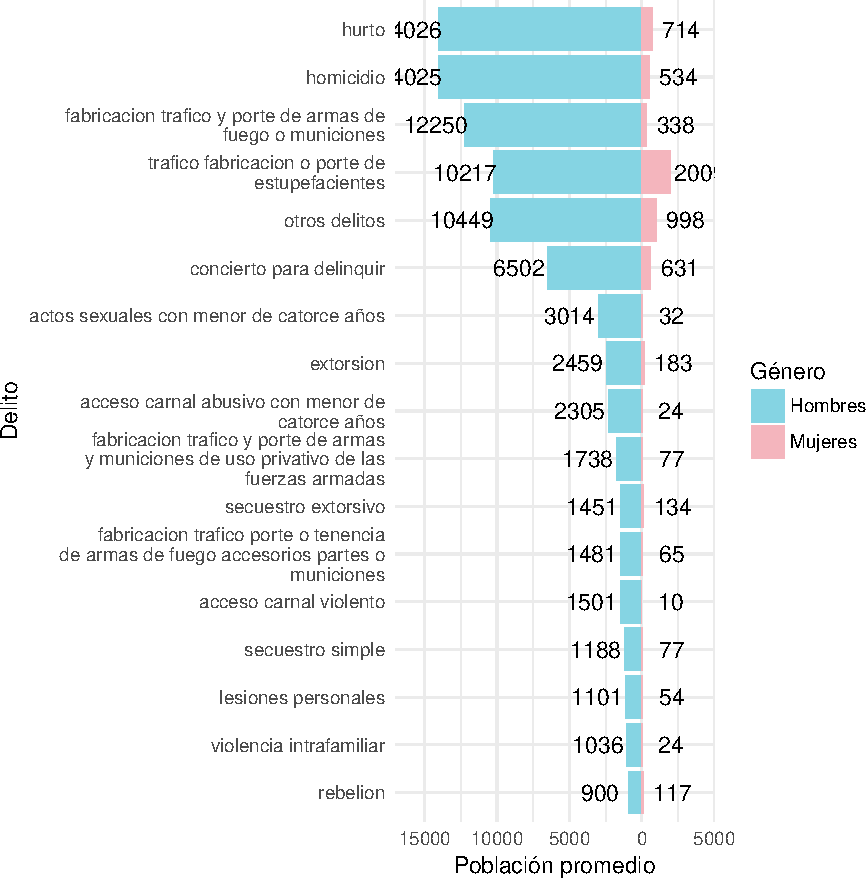
\includegraphics[width=0.7\linewidth]{delito-1.pdf}
	\caption{Poblaci�n carcelaria promedio por delito y g�nero. Julio 2013-Diciembre 2016} {Fuente: INPEC} {Elaboraci�n propia}
	\label{fig:delito}
\end{figure}

En la figura \ref{fig:delito} se observa la poblaci�n privada de la libertad promedio entre julio 2013 y diciembre 2016. Los delitos m�s comunes son: hurto; homicidio; fabricaci�n y porte de armas de fuego o municiones; tr�fico, fabricaci�n o porte de estupefacientes y concierto para delinquir. Tanto en hombres como mujeres estos cinco delitos son los m�s comunes; en los hombres se manifiestan en el orden presentado, pero en las mujeres los delitos m�s frecuentes son tr�fico, fabricaci�n o porte de estupefacientes y concierto para delinquir, seguidos por hurto, homicidio y fabricaci�n y porte de armas de fuego. 

Las figuras \ref{fig:delitoshombres} y \ref{fig:delitosmujeres} presentan la evoluci�n de la poblaci�n carcelaria por delito entre Julio 2013 y Diciembre 2016, para hombres y mujeres respectivamente. Las gr�ficas evidencian un comportamiento aparentemente independiente de las series: Por ejemplo:  mientras las series de hurto, extorsi�n y secuestro simple presentan un descenso de la poblaci�n condenada en 2014 y una posterior estabilizaci�n, concierto para delinquir presenta una tendencia al alza estable, tanto en sindicados como en condenados.


\begin{figure}[H]
	\centering
	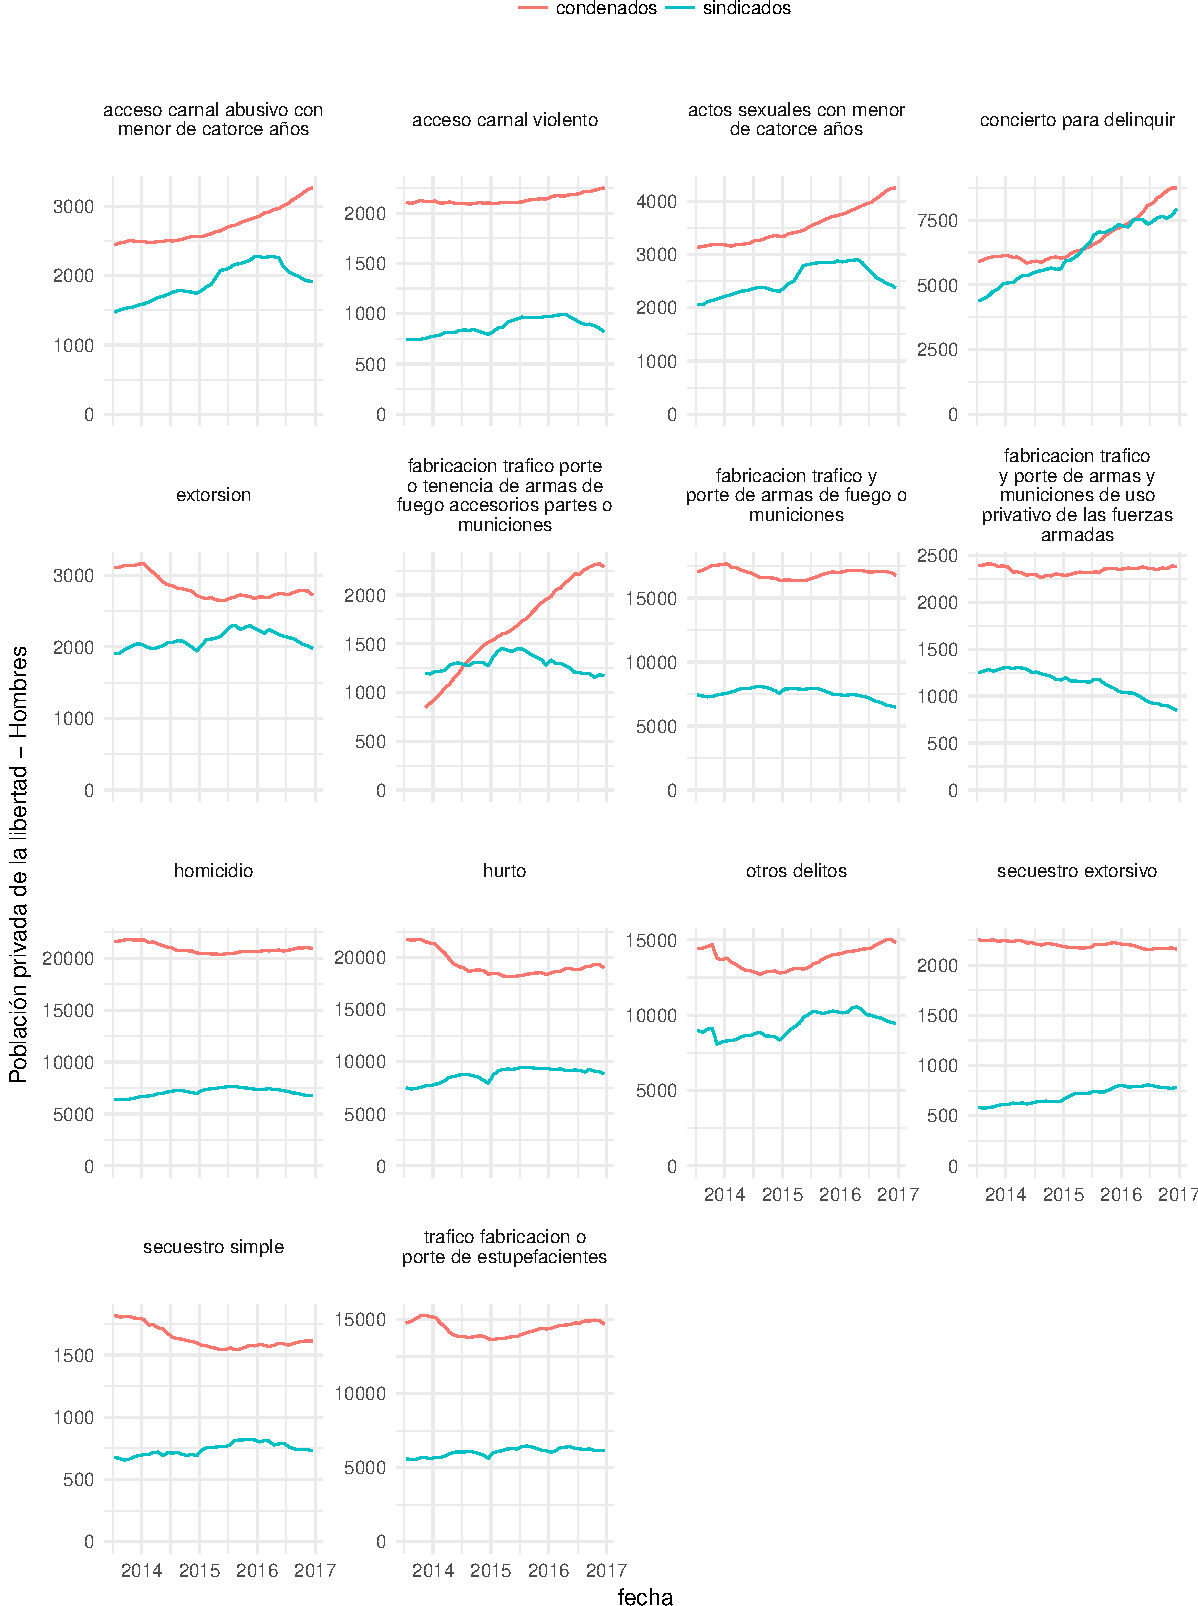
\includegraphics[width=1\linewidth]{delitoshombres-1.pdf}
	\caption{Evoluci�n de la poblaci�n carcelaria masculina, Julio 2013-Diciembre 2016} {Fuente: INPEC} {Elaboraci�n propia}
	\label{fig:delitoshombres}
\end{figure}

\begin{figure}[H]
	\centering
	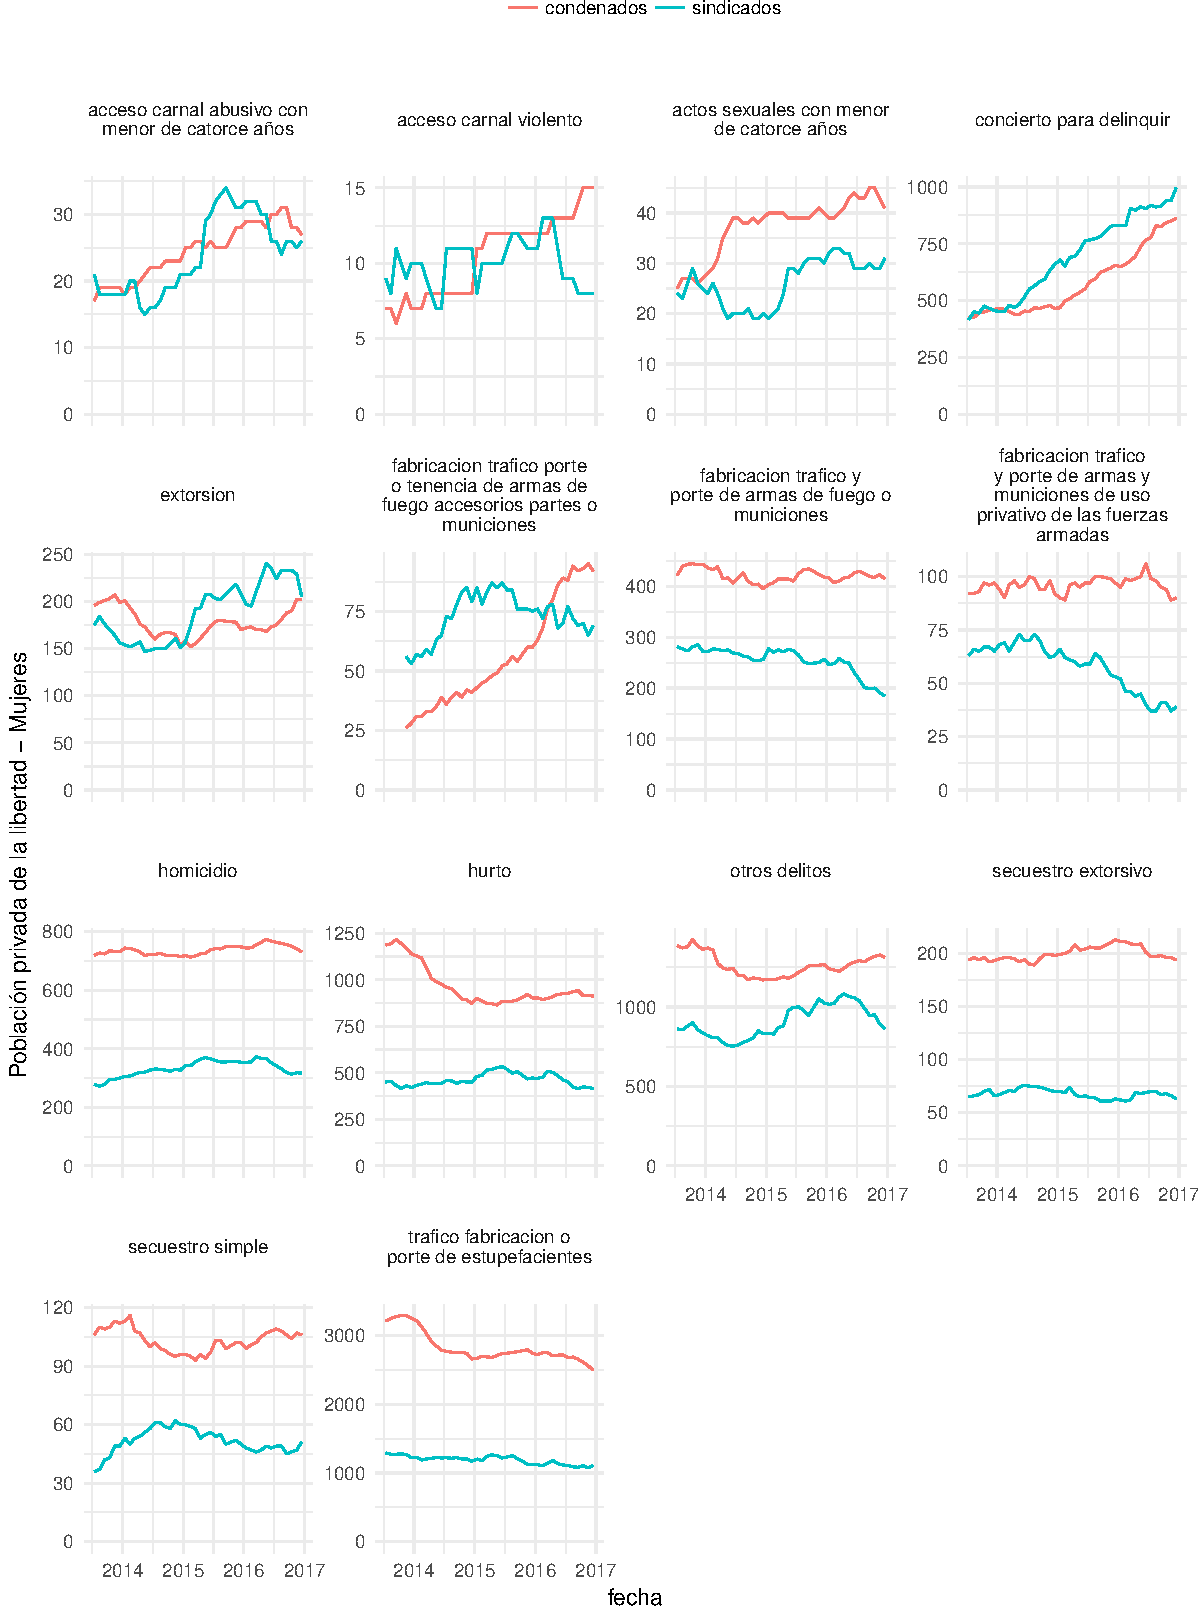
\includegraphics[width=1\linewidth]{delitosmujeres-1.pdf}
	\caption{Evoluci�n de la poblaci�n carcelaria femenina, Julio 2013-Diciembre 2016} {Fuente: INPEC} {Elaboraci�n propia}
	\label{fig:delitosmujeres}
\end{figure}

\section{Selecci�n de Software}

Para mantener un �nico ambiente de desarrollo, nos enfocamos en los paquetes desarrollados en R, como los mencionados por Petris \cite{Petris2011}, Helske \cite{Helske2017} y Tusell \cite{Tusell2011}. Dentro de los paquetes analizados se encuentran  \textit{Kfas} por Helske(2017) \cite{Helske2017} y \textit{MARSS} de Holmes(2018) \cite{Holmes2018}. Se utiliza \textit{MARSS} por la flexibilidad en la definici�n del modelo.

\section{Identificaci�n del modelo}

Holmes \& Ward \& Willis (2018) definen los modelos MARSS, Modelos auto-regresivos multivariados, de forma general como: 

\begin{equation}\label{estado}
\bm{x_{t}  = B_{t}x_{t-1} +u_t +C_tc_t +G_tw_t} \quad donde \quad \bm{w_t} \sim MVN(0,\bm{Q_t})
\end{equation}

\begin{equation}\label{observado}
\bm{y_{t} = Z_{t}x_{t} +a_{t} +D_{t}d_{t} +H_{t}v_{t}} \quad donde \quad \bm{v_t} \sim MVN(0,\bm{R_t})
\end{equation}

\begin{equation}
x_1 \sim MVN(\pi,\Lambda)\, o \, x_0 \sim MVN(\pi,\Lambda)
\end{equation}

$\bm{x}$ es una matriz de $m \times T$, donde cada $x_t$ es una realizaci�n de la variable aleatoria $X_t$ en el instante $t$. $m$ se considera la cantidad de variables latentes. 

$\bm{w}$ es el error de proceso y es un vector aleatorio de dimensi�n $m \times T$ con distribuci�n normal multivariada (MVN) de media cero y matriz de varianzas y covarianzas $\bm{Q}$.

$\bm{y}$ es una matriz de $n \times T$, con T observaciones. Algunas observaciones pueden ser faltantes. $n$ se considera la cantidad de variables observadas.

$\bm{v}$ es el error de observaci�n de tama�o $n \times T$, con media cero y varianza $\bm{R}$

$\bm{B_t}$ y $\bm{Z_t}$ son par�metros y son de dimensi�n $m \times m$ y $n \times m$. 

$\bm{u_t}$ y $\bm{a_t}$ son par�metros de vectores de dimensi�n $m \times T$ y $n \times T$.

$\bm{Q_t}$ y $\bm{R_t}$ son matrices de varianzas y covarianzas de tama�o  $m \times m$ y $n \times n$.

$\pi$ y $\Lambda$ son par�metros o son fijados con antelaci�n.

$\bm{C_t}$ y $\bm{D_t}$ son matrices de par�metros de tama�o  $m \times p$ y $n \times q$.

$\bm{c}$ y $\bm{d}$ son inputs, $p$ y $q$ variables ex�genas, sin datos faltantes, de dimensi�n $p \times T$
 y $ q \times T$.
 
$\bm{G_t}$ y $\bm{H_t}$ son inputs, matrices de tama�o   $m \times g$ y $n \times h$.

En este cap�tulo se analizar� un modelo bivariado, donde $\bm{x_t}$ corresponde a la poblaci�n sindicada y condenada. Se restringe el modelo con las siguientes consideraciones: 

\begin{itemize}
	\item No hay una interacci�n entre la poblaci�n de sindicados en el periodo $t$, y la poblaci�n de condenados el periodo $t-1$. Es decir se modelo que no hay paso de condenados a sindicados. 
	\item La observaci�n $y_t$ se considera una insesgada frente al valor de la variable $x_t$. Esto implica $a_t = 0$ y  $v_t \sim MVN(0,R) $. 
	\item La poblaci�n condenada en el periodo t depende solamente de la poblaci�n en el periodo sindicada y condenada en el periodo t-1. $U2_t = 0$. Las salidas son proporcionales a la poblaci�n condenada $0 \leq b4 \leq 1$.
\end{itemize}

\begin{equation}
\begin{bmatrix} X_{1,t}  \\ X_{2,t} \end{bmatrix} =
\begin{bmatrix}
b1 & 0 \\
b2 & b4 &
\end{bmatrix} 
\begin{bmatrix} X_{1,t-1}  \\ X_{2,t-1} \end{bmatrix} +
\begin{bmatrix} U_{1}  \\ 0 \end{bmatrix} +
\begin{bmatrix} w_{1,t}  \\ w_{2,t} \end{bmatrix}, \begin{bmatrix} w_{1,t}  \\ w_{2,t} \end{bmatrix} \sim MVN(\begin{bmatrix} 0  \\ 0 \end{bmatrix},  \begin{bmatrix} Q_{11}  &  Q_{12} \\ Q_{12} & Q_{22}\end{bmatrix})
\end{equation}

\begin{equation}
\begin{bmatrix} Y_{1,t} \\ Y_{2,t} \end{bmatrix} =
\begin{bmatrix}
1 & 0 \\ 0 & 1
\end{bmatrix} 
\begin{bmatrix} X_{1,t-1}  \\ X_{2,t-1} \end{bmatrix} +
\begin{bmatrix} v_{1,t}  \\ v_{2,t} \end{bmatrix} , \begin{bmatrix} v_{1,t}  \\ v_{2,t} \end{bmatrix} \sim MVN(\begin{bmatrix} 0  \\ 0 \end{bmatrix},  \begin{bmatrix} R_{11} &  R_{12} \\ R_{12} & R_{22} \end{bmatrix})
\label{equ:observado}
\end{equation}

Donde 

$X_{1,t}$ = Poblaci�n sindicada en el periodo t

$X_{2,t}$ = Poblaci�n condenada en el periodo t

$b_{1}$ = Efecto en la poblaci�n sindicada en el periodo $t-1$ en la poblaci�n sindicada en el periodo $t$

$b_{2}$ = Efecto en la poblaci�n sindicada en el periodo $t-1$ en la poblaci�n condenada en el periodo $t$

$b_{4}$ = Efecto en la poblaci�n condenada en el periodo $t-1$ en la poblaci�n condenada en el periodo $t$.

$b_{4}$ = Poblaci�n condenada en el periodo t

$U_{1}$ = Variaci�n constante mensual en la poblaci�n sindicada no asociada a la poblaci�n sindicada en el periodo anterior.

$Y_{1,t}$ = Poblaci�n sindicada observada en el periodo t

$Y_{2_t}$ = Poblaci�n condenada observada en el periodo t

$w_1$, $w_2$, $v_1$, $v_2$,$\bm{Q}$, $\bm{R}$  mantienen el mismo sentido que en las ecuaciones \ref{estado} y \ref{observado}

Modelar el sistema a partir de este modelo te�rico, nos permite estimar sus par�metros usando el paquete MARSS. Tratar la serie como un modelo estado-espacio tambi�n permite tratar los faltantes con facilidad.

En el ejercicio con datos reales se ajust� un segundo modelo con una variable Dummy $\bm{c}$ en 2014, debido al efecto de los cambios normativos en la tendencia de la poblaci�n. 

\section{Estimaci�n de par�metros}

La estimaci�n se realiza en series bivariadas por delito, g�nero. Se presenta en detalle procedimiento para la serie de hurto en hombres, en series adicionales se presentan resultados de la proyecci�n. La estimaci�n de los par�metros se realiza con el paquete MARSS, que utiliza el algoritmo EM para realizar la estimaci�n. La estimaci�n de los estados se realiza por suavizamiento. 

Una variable Dummy correspondiente a 2014 se agreg� al modelo. En este periodo se detuvo el crecimiento de la poblaci�n carcelaria gracias a la entrada en vigor de la ley 1709 de 2014. Dos mediciones del impacto de la ley 1709 son realizadas por el INPEC en 2014, se�alando el cambio observado en la tendencia de la poblaci�n carcelaria \cite{OficinaAsesoradePlaneacion2014} \cite{Asesora2014}. Las gr�ficas \ref{fig:delitoshombres} y \ref{fig:delitosmujeres} muestran que en 2015 y 2016 la poblaci�n carcelaria regresa a su comportamiento usual.

% latex table generated in R 3.4.4 by xtable 1.8-2 package
% Mon Jun 11 23:12:33 2018
\begin{table}[ht]
	\centering
	\begin{tabular}{rr}
		\hline
		& x \\ 
		\hline
		b1 & 0.94 \\ 
		b2 & 0.05 \\ 
		b4 & 0.98 \\ 
		U1 & 514.58 \\ 
		q11 & 23317.33 \\ 
		q12 & -11076.07 \\ 
		q22 & 18110.12 \\ 
		\hline
	\end{tabular}
	\caption{Par�metros estimados: hurto, hombres} {Fuente: INPEC} {Elaboraci�n propia}
	\label{tab:Estimadoshurtohombres}
\end{table}

\begin{figure}[H]
	\centering
	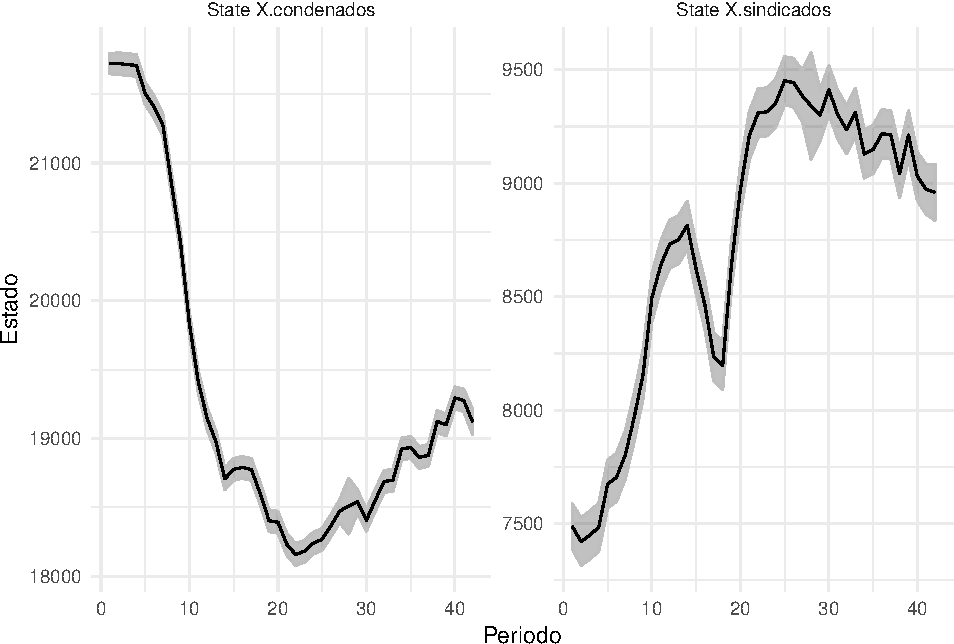
\includegraphics[width=0.7\linewidth]{ajuste_hurtos-1.pdf}
	\caption{Poblaci�n sindicada y condenada por hurto, hombres} {Fuente: INPEC} {Elaboraci�n propia}
	\label{fig:estadoespacioinputa}
\end{figure}

\begin{figure}[H]
	\centering
	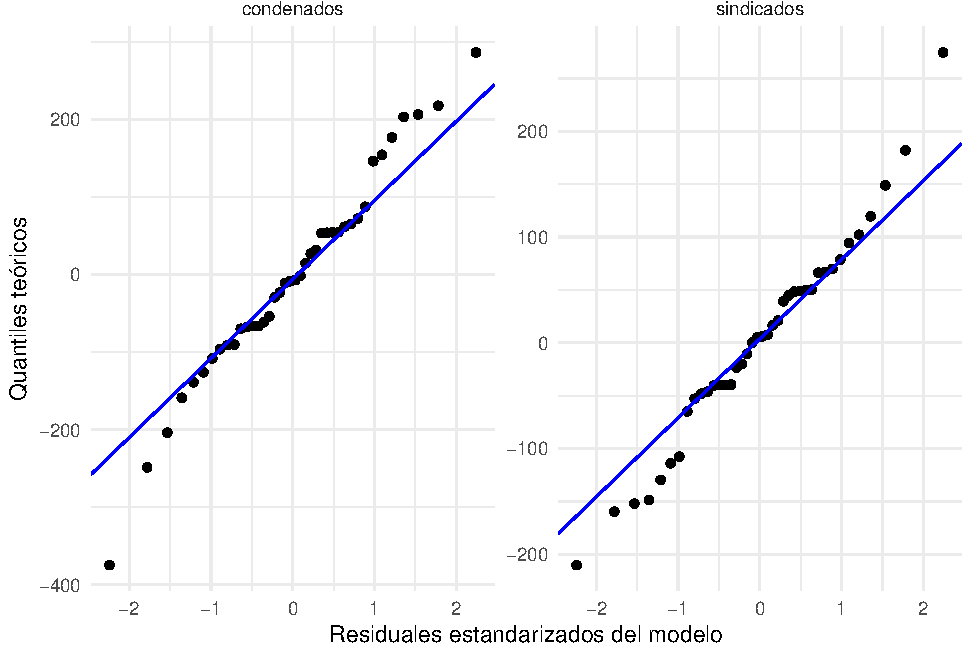
\includegraphics[width=0.7\linewidth]{ajuste_hurtos-2.pdf}
	\caption{Poblaci�n carcelaria promedio por delito y g�nero. Octubre 2013-Diciembre 2016} {Fuente: INPEC} {Elaboraci�n propia}
	\label{fig:estadoespacioqqplot}
\end{figure}

\begin{figure}[H]
	\centering
	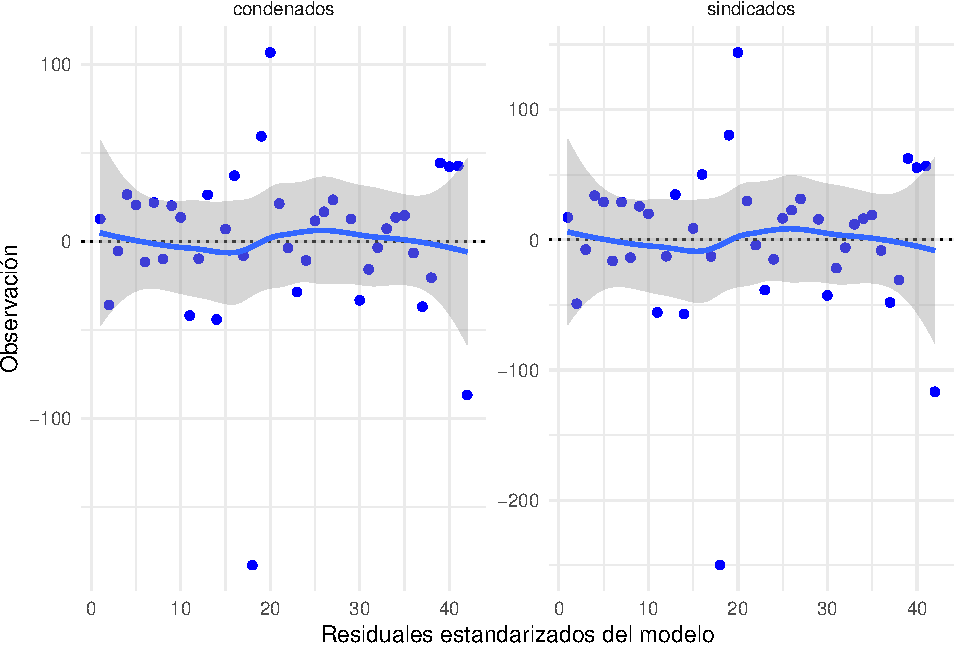
\includegraphics[width=0.7\linewidth]{ajuste_hurtos-3.pdf}
	\caption{Poblaci�n carcelaria promedio por delito y g�nero. Octubre 2013-Diciembre 2016} {Fuente: INPEC} {Elaboraci�n propia}
	\label{fig:estadoespacioerror}
\end{figure}

El qqplot sugiere un comportamiento normal del error con presencia de datos at�picos. La gr�fica muestra rachas de puntos arriba y abajo de cero, lo que sugiere la presencia de autocorrelaci�n en el error. Esta aparente autocorrelaci�n puede estar asociada a componentes estacionales o cambios estructurales.


\section{Proyecciones 2017 - 2020}

Se realiza proyecci�n de la poblaci�n media sindicada y condenada en la tabla \ref{tab:Estimadoshurtohombres}

% latex table generated in R 3.4.4 by xtable 1.8-2 package
% Mon Jun 11 23:17:58 2018
\begin{table}[H]
	\centering
	\begin{tabular}{rlrr}
		\hline
		& Periodo & Sindicados & Condenados \\ 
		\hline
		V1 & 2017-01-15 & 8862.00 & 19050.00 \\ 
		V2 & 2017-02-15 & 8880.00 & 19067.00 \\ 
		V3 & 2017-03-15 & 8897.00 & 19085.00 \\ 
		V4 & 2017-04-15 & 8913.00 & 19103.00 \\ 
		V5 & 2017-05-15 & 8929.00 & 19121.00 \\ 
		V6 & 2017-06-15 & 8943.00 & 19140.00 \\ 
		V7 & 2017-07-15 & 8956.00 & 19159.00 \\ 
		V8 & 2017-08-15 & 8969.00 & 19178.00 \\ 
		V9 & 2017-09-15 & 8981.00 & 19198.00 \\ 
		V10 & 2017-10-15 & 8993.00 & 19217.00 \\ 
		V11 & 2017-11-15 & 9003.00 & 19237.00 \\ 
		V12 & 2017-12-15 & 9014.00 & 19257.00 \\ 
		V13 & 2018-01-15 & 9023.00 & 19277.00 \\ 
		V14 & 2018-02-15 & 9032.00 & 19297.00 \\ 
		V15 & 2018-03-15 & 9041.00 & 19317.00 \\ 
		V16 & 2018-04-15 & 9049.00 & 19337.00 \\ 
		V17 & 2018-05-15 & 9056.00 & 19357.00 \\ 
		V18 & 2018-06-15 & 9064.00 & 19377.00 \\ 
		V19 & 2018-07-15 & 9070.00 & 19397.00 \\ 
		V20 & 2018-08-15 & 9077.00 & 19417.00 \\ 
		V21 & 2018-09-15 & 9083.00 & 19436.00 \\ 
		V22 & 2018-10-15 & 9089.00 & 19456.00 \\ 
		V23 & 2018-11-15 & 9094.00 & 19475.00 \\ 
		V24 & 2018-12-15 & 9099.00 & 19494.00 \\ 
		V25 & 2019-01-15 & 9104.00 & 19513.00 \\ 
		V26 & 2019-02-15 & 9108.00 & 19532.00 \\ 
		V27 & 2019-03-15 & 9113.00 & 19550.00 \\ 
		V28 & 2019-04-15 & 9117.00 & 19569.00 \\ 
		V29 & 2019-05-15 & 9120.00 & 19587.00 \\ 
		V30 & 2019-06-15 & 9124.00 & 19605.00 \\ 
		V31 & 2019-07-15 & 9127.00 & 19622.00 \\ 
		V32 & 2019-08-15 & 9131.00 & 19640.00 \\ 
		V33 & 2019-09-15 & 9134.00 & 19657.00 \\ 
		V34 & 2019-10-15 & 9137.00 & 19674.00 \\ 
		V35 & 2019-11-15 & 9139.00 & 19690.00 \\ 
		V36 & 2019-12-15 & 9142.00 & 19707.00 \\ 
		\hline
	\end{tabular}
	\caption{Proyecci�n a treinta y seis meses: hurto, hombres} {Fuente: INPEC} {Elaboraci�n propia}
	\label{tab:Estimadoshurtohombres}
\end{table}

% latex table generated in R 3.4.4 by xtable 1.8-2 package
% Tue Jun 12 01:05:12 2018
\begin{table}[H]
	\centering
	\begin{tabular}{rllrrr}
		\hline
		& Periodo & G�nero & Sindicados & Condenados & Total \\ 
		\hline
		1 & 2017-01-15 & Hombres & 56331 & 116190 & 172521 \\ 
		2 & 2017-02-15 & Hombres & 56393 & 116397 & 172790 \\ 
		3 & 2017-03-15 & Hombres & 56447 & 116603 & 173050 \\ 
		4 & 2017-04-15 & Hombres & 56495 & 116807 & 173302 \\ 
		5 & 2017-05-15 & Hombres & 56536 & 117009 & 173544 \\ 
		6 & 2017-06-15 & Hombres & 56570 & 117208 & 173778 \\ 
		7 & 2017-07-15 & Hombres & 56598 & 117405 & 174003 \\ 
		8 & 2017-08-15 & Hombres & 56619 & 117599 & 174218 \\ 
		9 & 2017-09-15 & Hombres & 56634 & 117790 & 174424 \\ 
		10 & 2017-10-15 & Hombres & 56643 & 117978 & 174621 \\ 
		11 & 2017-11-15 & Hombres & 56646 & 118163 & 174809 \\ 
		12 & 2017-12-15 & Hombres & 56642 & 118344 & 174987 \\ 
		13 & 2018-01-15 & Hombres & 56633 & 118522 & 175155 \\ 
		14 & 2018-02-15 & Hombres & 56618 & 118696 & 175314 \\ 
		15 & 2018-03-15 & Hombres & 56596 & 118866 & 175462 \\ 
		16 & 2018-04-15 & Hombres & 56569 & 119032 & 175601 \\ 
		17 & 2018-05-15 & Hombres & 56535 & 119195 & 175730 \\ 
		18 & 2018-06-15 & Hombres & 56496 & 119353 & 175849 \\ 
		19 & 2018-07-15 & Hombres & 56450 & 119507 & 175957 \\ 
		20 & 2018-08-15 & Hombres & 56398 & 119657 & 176055 \\ 
		21 & 2018-09-15 & Hombres & 56340 & 119802 & 176142 \\ 
		22 & 2018-10-15 & Hombres & 56276 & 119943 & 176219 \\ 
		23 & 2018-11-15 & Hombres & 56262 & 120080 & 176342 \\ 
		24 & 2018-12-15 & Hombres & 56251 & 120212 & 176463 \\ 
		25 & 2019-01-15 & Hombres & 56236 & 120340 & 176576 \\ 
		26 & 2019-02-15 & Hombres & 56219 & 120463 & 176681 \\ 
		27 & 2019-03-15 & Hombres & 56197 & 120581 & 176779 \\ 
		28 & 2019-04-15 & Hombres & 56173 & 120695 & 176868 \\ 
		29 & 2019-05-15 & Hombres & 56145 & 120805 & 176949 \\ 
		30 & 2019-06-15 & Hombres & 56114 & 120909 & 177023 \\ 
		31 & 2019-07-15 & Hombres & 56080 & 121009 & 177088 \\ 
		32 & 2019-08-15 & Hombres & 56042 & 121104 & 177146 \\ 
		33 & 2019-09-15 & Hombres & 56001 & 121194 & 177196 \\ 
		34 & 2019-10-15 & Hombres & 55957 & 121280 & 177237 \\ 
		35 & 2019-11-15 & Hombres & 55910 & 121361 & 177271 \\ 
		36 & 2019-12-15 & Hombres & 55860 & 121437 & 177296 \\ 
		\hline
	\end{tabular}
	\caption{Proyecci�n de la poblaci�n carcelaria total, hombres} {Fuente: INPEC} {Elaboraci�n propia}
	\label{tab:Pryhombres}
\end{table}

% latex table generated in R 3.4.4 by xtable 1.8-2 package
% Tue Jun 12 01:05:12 2018

\begin{table}[H]
	\centering
	\begin{tabular}{rllrrr}
		\hline
		& Periodo & G�nero & Sindicados & Condenados & Total \\ 
		\hline
		1 & 2017-01-15 & Mujeres & 4396 & 7511 & 11907 \\ 
		2 & 2017-02-15 & Mujeres & 4413 & 7528 & 11941 \\ 
		3 & 2017-03-15 & Mujeres & 4429 & 7544 & 11973 \\ 
		4 & 2017-04-15 & Mujeres & 4446 & 7560 & 12005 \\ 
		5 & 2017-05-15 & Mujeres & 4461 & 7575 & 12037 \\ 
		6 & 2017-06-15 & Mujeres & 4477 & 7591 & 12068 \\ 
		7 & 2017-07-15 & Mujeres & 4492 & 7606 & 12098 \\ 
		8 & 2017-08-15 & Mujeres & 4507 & 7621 & 12128 \\ 
		9 & 2017-09-15 & Mujeres & 4523 & 7635 & 12158 \\ 
		10 & 2017-10-15 & Mujeres & 4538 & 7650 & 12187 \\ 
		11 & 2017-11-15 & Mujeres & 4552 & 7664 & 12217 \\ 
		12 & 2017-12-15 & Mujeres & 4567 & 7679 & 12246 \\ 
		13 & 2018-01-15 & Mujeres & 4582 & 7693 & 12275 \\ 
		14 & 2018-02-15 & Mujeres & 4597 & 7707 & 12304 \\ 
		15 & 2018-03-15 & Mujeres & 4612 & 7721 & 12334 \\ 
		16 & 2018-04-15 & Mujeres & 4628 & 7736 & 12363 \\ 
		17 & 2018-05-15 & Mujeres & 4643 & 7750 & 12393 \\ 
		18 & 2018-06-15 & Mujeres & 4658 & 7764 & 12423 \\ 
		19 & 2018-07-15 & Mujeres & 4674 & 7779 & 12452 \\ 
		20 & 2018-08-15 & Mujeres & 4689 & 7793 & 12483 \\ 
		21 & 2018-09-15 & Mujeres & 4705 & 7808 & 12513 \\ 
		22 & 2018-10-15 & Mujeres & 4721 & 7823 & 12544 \\ 
		23 & 2018-11-15 & Mujeres & 4737 & 7838 & 12575 \\ 
		24 & 2018-12-15 & Mujeres & 4754 & 7852 & 12606 \\ 
		25 & 2019-01-15 & Mujeres & 4770 & 7868 & 12638 \\ 
		26 & 2019-02-15 & Mujeres & 4787 & 7883 & 12670 \\ 
		27 & 2019-03-15 & Mujeres & 4804 & 7898 & 12703 \\ 
		28 & 2019-04-15 & Mujeres & 4822 & 7914 & 12736 \\ 
		29 & 2019-05-15 & Mujeres & 4839 & 7930 & 12769 \\ 
		30 & 2019-06-15 & Mujeres & 4857 & 7946 & 12803 \\ 
		31 & 2019-07-15 & Mujeres & 4875 & 7962 & 12837 \\ 
		32 & 2019-08-15 & Mujeres & 4894 & 7978 & 12872 \\ 
		33 & 2019-09-15 & Mujeres & 4913 & 7995 & 12907 \\ 
		34 & 2019-10-15 & Mujeres & 4932 & 8011 & 12943 \\ 
		35 & 2019-11-15 & Mujeres & 4951 & 8028 & 12979 \\ 
		36 & 2019-12-15 & Mujeres & 4971 & 8045 & 13016 \\ 
		\hline
	\end{tabular}
	\caption{Proyecci�n de la poblaci�n carcelaria total, mujeres} {Fuente: INPEC} {Elaboraci�n propia}
	\label{tab:Prymujeres}
\end{table}

La proyecci�n de la poblaci�n total se obtiene como la suma de las proyecciones por delito. Proyecciones par hombres y mujeres se presentan en las tablas \ref{tab:Pryhombres} y \ref{tab:Prymujeres}. Las gr�ficas \ref{fig:prydelitoshombres} y \ref{fig:prydelitosmujeres} presentan la proyecci�n por delito. Las proyecciones son coherentes con el comportamiento hist�rico de cada serie. En fabricaci�n, tr�fico y porte de armas y municiones de uso privativo de las fuerzas armadas no resulta coherente la proyecci�n, pues presenta una serie de sindicados que cae a cero y una serie de condenados que continua creciendo luego, para resolver este inconveniente se podr�an restringir los par�metros del modelo, tal que $0 \leq b1, b2, b3 \leq 1$.

\begin{figure}[H]
	\centering
	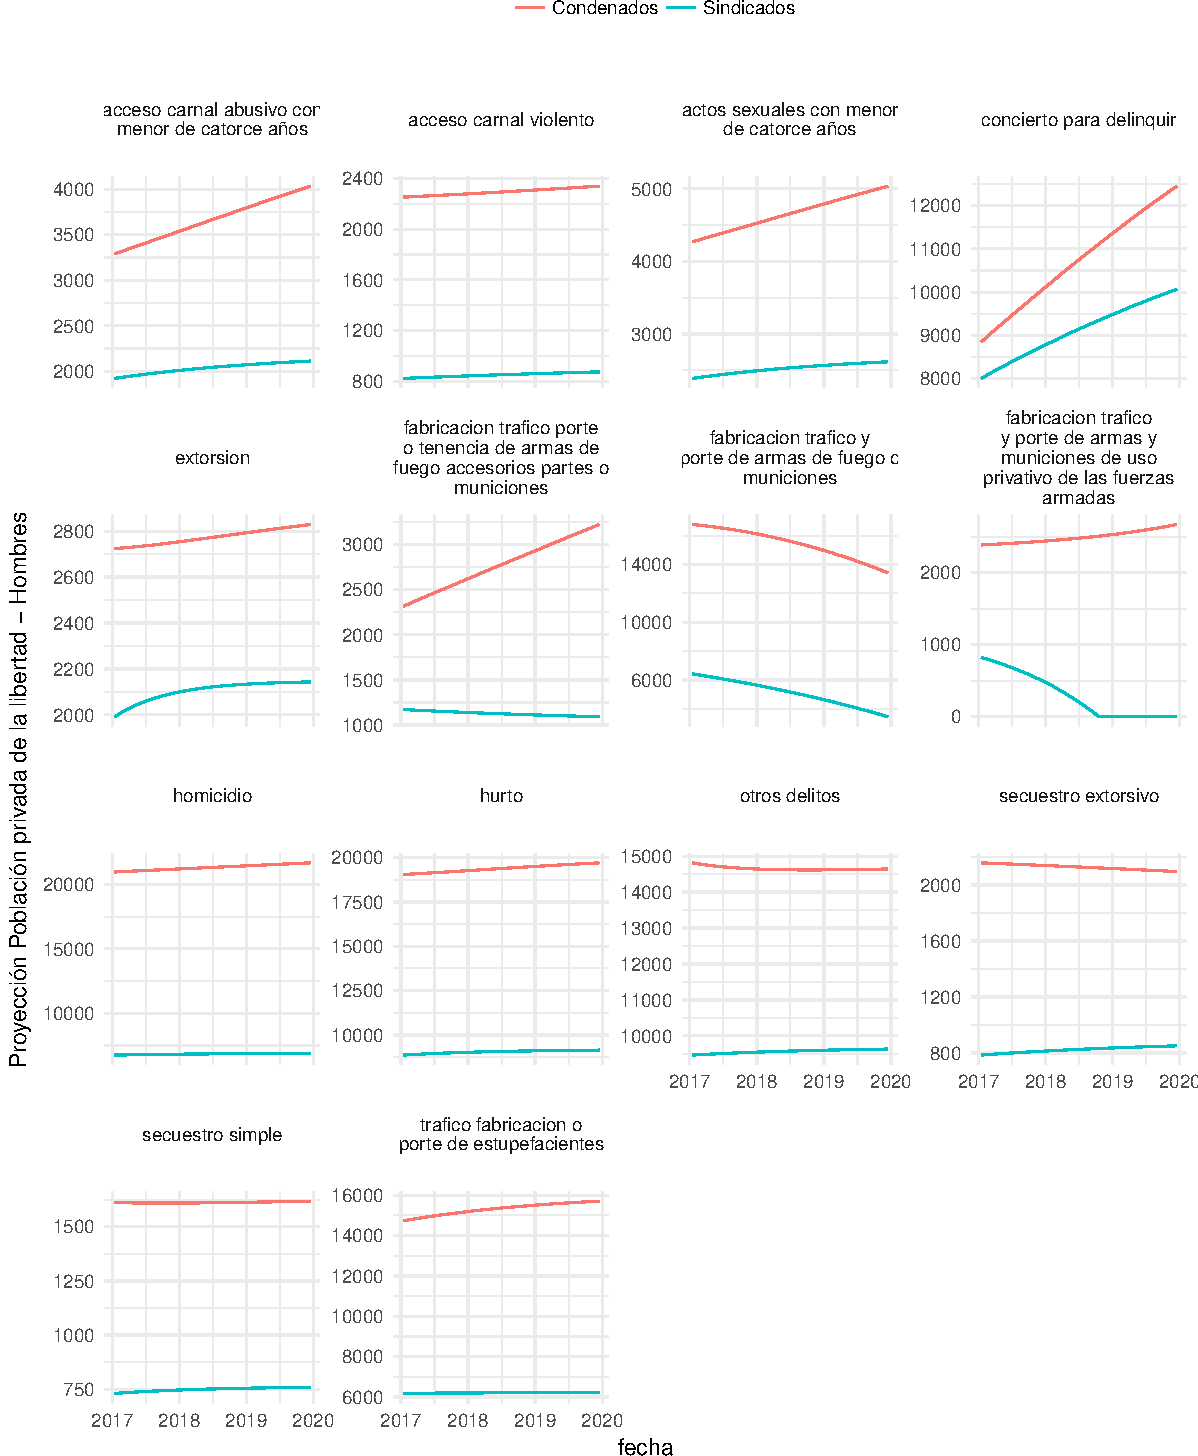
\includegraphics[width=1\linewidth]{pry_delitos_hombres-1.pdf}
	\caption{Proyecci�n de poblaci�n carcelaria o por delito, hombres  2017 - 2020} {Fuente: INPEC} {Elaboraci�n propia}
	\label{fig:prydelitoshombres}
\end{figure}


\begin{figure}[H]
	\centering
	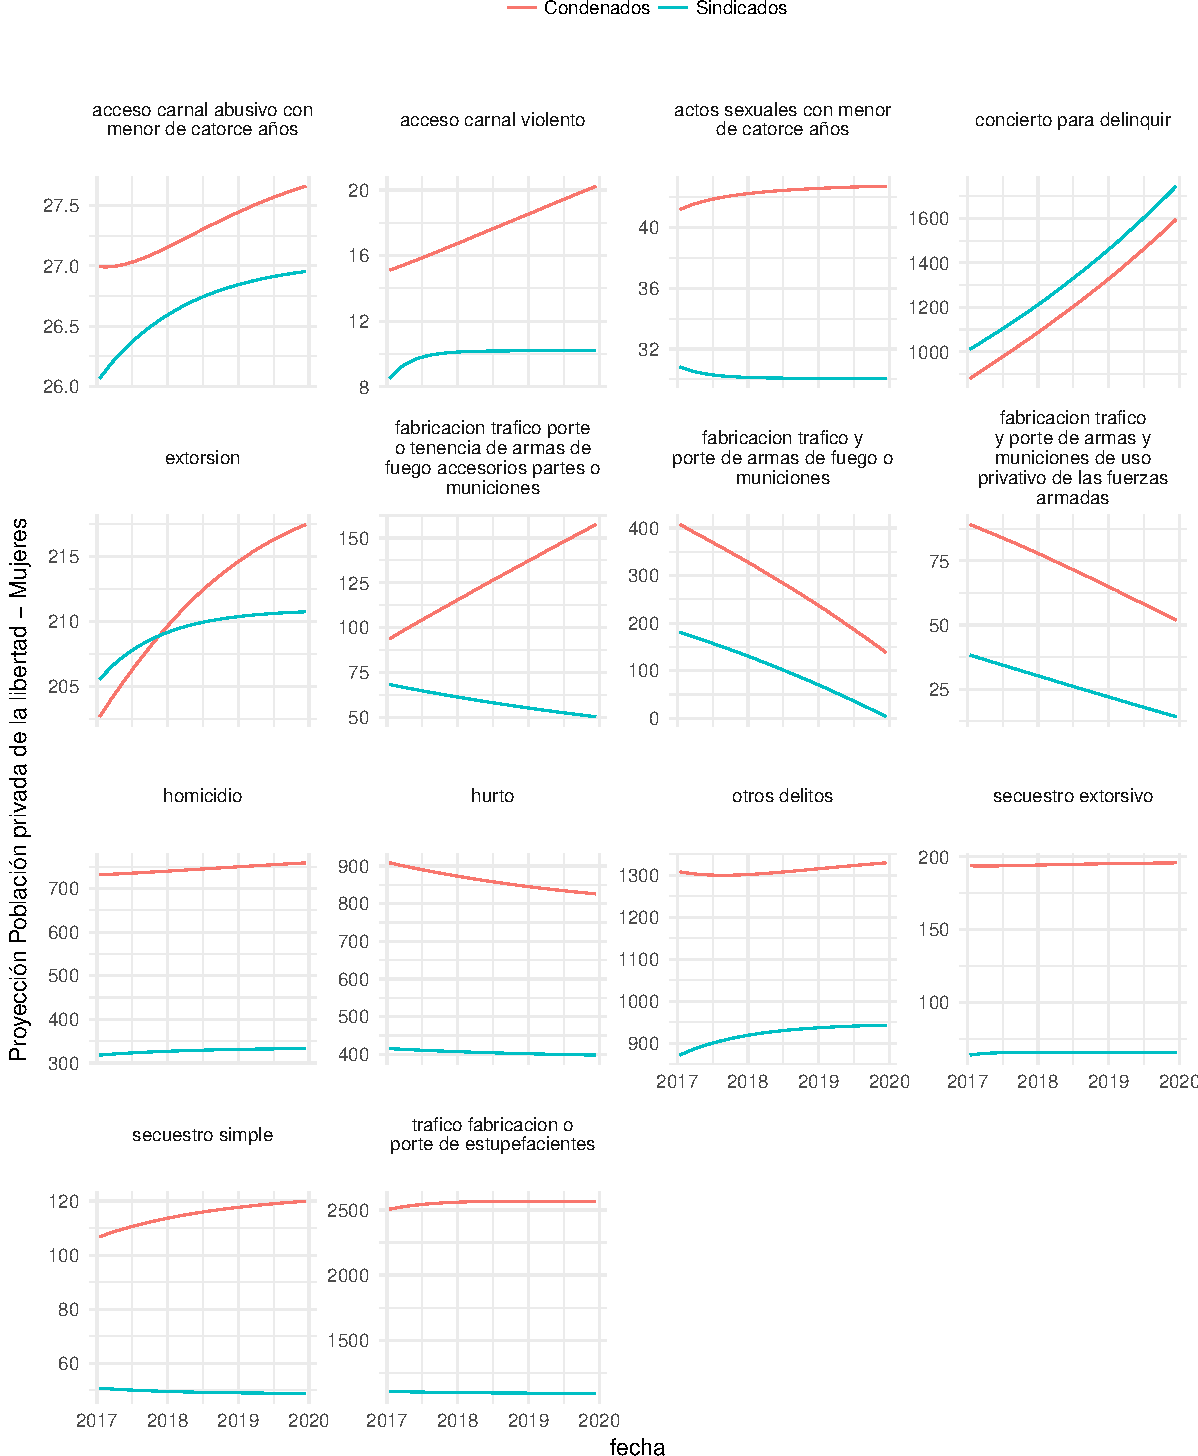
\includegraphics[width=1\linewidth]{pry_delitos_mujeres-1.pdf}
	\caption{Proyecci�n de poblaci�n carcelaria o por delito, mujeres  2017 - 2020} {Fuente: INPEC} {Elaboraci�n propia}
	\label{fig:prydelitosmujeres}
\end{figure}

\section{Discusi�n}

Los modelos estado-espacio son una herramienta potente que permite estimar modelos interpretables en series de tiempo, incluso con variables no observadas, como las sentencias y en presencia de datos faltantes.El desarrollo de paquetes en R que permitan realizar estimaciones de m�xima verosimilitud bajo restricciones en los par�metros, en forma simple, como la trabajada en el paquete MARSS quedan dentro de trabajo futuro. Por ejemplo restringir los par�metros $b1$ y $b2$ a ser valores entre cero y uno.

Tratar cada delito como una poblaci�n separada, considerando la interacci�n entre la poblaci�n sindicada y condenada permite analizar la 
tendencia y variabilidad de cada serie. En este cap�tulo se evidenci� comportamientos diferentes para cada serie en tendencia y variabilidad, con algunos componentes compartidos, como el efecto de los cambios de regulaci�n en 2014 orientados a reducir la poblaci�n carcelaria.

Al imponer un modelo te�rico en todas las series de delitos, se puede perder informaci�n espec�fica de las series de delitos. Como trabajo futuro est� analizar el comportamiento individual de cada serie, y sus cambios estructurales. 

La longitud de la serie disponible no permite estimar un comportamiento estacional, y en consecuencia dificulta separar los efectos estacionales de cambios de r�gimen. En cada delito se presentan errores at�picos, donde no se puede asignar a un componente estacional, o a cambios en la reglamentaci�n.

El modelo no incluye en principio el efecto de la estructura etaria, as� que puede resultar menos efectivo en el largo plazo que los modelos de poblaciones peque�as.

	%\appendix
	%    \chapter{Gr�ficas adicionales}

\begin{figure}[htb]
 \centering
 
\includegraphics[width=10cm]{small_escudo_color}
 \caption{Escudo oficial de la UN a color dise�ado por el Maestro Francisco Duarte.}
 \label{fig:escudo_color}
\end{figure}


\begin{table}
\centering
\caption{Unidades de \TeX.}
\begin{tabular}{l|l}\hline
\verb"mm" & mil�metro $\approx$ 1/25 pulgada \\
\verb"cm" & cent�metro = 10 mm \\
\verb"in" & pulgada $\approx$ 25 mm \\
\verb"pt" & punto $\approx$ 1/72 pulgada $\approx$ 1/3 mm \\
\verb"em" & aprox. el ancho de una m en el tipo actual \\
\verb"ex" & aprox. la altura de una x en el tipo actual \\\hline
\end{tabular}
\end{table}

\begin{table}
\centering\renewcommand{\arraystretch}{2}
\caption{Tama�os de los tipos de fuentes \LaTeX.}
 \begin{tabular}{ll|ll}\hline
{\tiny\verb"\tiny"} & {\tiny letra diminuta}
& {\large\verb"\large"} & {\large letra grande} \\
{\scriptsize\verb"\scriptsize"} & {\scriptsize letra muy peque�a}
& {\Large\verb"\Large"} & {\Large letra mayor} \\
{\footnotesize\verb"\footnotesize"} & {\footnotesize letra bastante peque�a}
& {\LARGE\verb"\LARGE"} & {\LARGE muy grande} \\
{\small\verb"\small"} & {\small letra peque�a}
& {\huge\verb"\huge"} & {\huge enorme} \\
\verb"\normalsize" & letra normal
& {\Huge\verb"\Huge"} & {\Huge la mayor} \\\hline
 \end{tabular}
\end{table}





	\backmatter
	\conclusion{conclusiones}
	\futurework{trabajofuturo}
	%    \glossary{glosario}
	%\nocite{*}
	\bibliography{references}
	%\printindex
\end{document}